%%%%%%%%%%%%%%%%%%%%%%%%%%%%%%%%%%%%%%%%%%%%%%%%%%

% Latex Kapitel erstellen. 
% 		Kopiere 'texPandoc/*.tex' nach 'content/tex' 
% 		'content/tex' **Handarbeit... für opt. Ergebnisse!** 
% 		Kopiere 'archiv/inhalt.tex' nach 'content/' 
% 		make -- Latex-PDF erstellen 
% ju 19-3-22 inhalt.tex

%%%%%%%%%%%%%%%%%%%%%%%%%%%%%%%%%%%%%%%%%%%%%%%%%%

% content/
\chapter{Grundlagen - Elektrik 1}
%ju 28-Mai-22 01-Grundlagen-Elektrik.tex
\section{Die elektrische Spannung}\label{die-elektrische-spannung}

\textbf{Spannung} $U \quad \text{[Volt]} \quad [V]$

\emph{italienischer Physiker Alessandro Volta (1745-1827)}

\begin{table}[!ht]% hier: !ht 
\centering 
	\caption{}% \label{tab:}%% anpassen 
\begin{tabular}{@{}llll@{}}
\hline
\textbf{Einheit} & \textbf{Abk.} & \textbf{Zahl} &
\textbf{Exponentialschreibweise} \\
\hline
kilo V & $[KV]$ & $1000~V$ & $\num{1,0e3}~V$ \\
Volt & $[V]$ & $1~V$ & $\num{1,0e0}~V$ \\
milli V & $[mV]$ & $0,001~V$ & $\num{1,0e-3}~V$ \\
\hline
\end{tabular} 
\end{table}

In einer Spannungsquelle, z.~B. Drehstromgenerator, werden die
unterschiedlichen Ladungen unter Energieaufwand (Drehbewegung,
Magnetismus) voneinander getrennt.

Es bilden sich zwei Pole aus.

\begin{itemize}
\item
  Negativer Pol: hier herrscht Elektronenüberschuss
\item
  Positiver Pol: Elektronenmangel
\end{itemize}

Man spricht hierbei auch von dem Vorhandensein einer Potentialdifferenz.

Diese beiden Ladungen haben das Bestreben sich auszugleichen, dieses
Ausgleichsbestreben bezeichnet man als elektrische Spannung.

\textbf{Messen}

Das Spannungsmessgerät wird grundsätzlich parallel zum Messobjekt
geschaltet.

\emph{Besonderheit}: Spannungsmessgeräte besitzen ein sehr hochohmigen
Innenwiderstand (Impedanz).

\newpage

\section{Der elektrische Strom}\label{der-elektrische-strom}

\textbf{Strom} $I \quad \text{[Ampere]} \quad [A]$

\emph{französischer Physiker André-Marie Ampère (1775-1836)}

I = Intensität, International >>Ampere<<

\begin{table}[!ht]% hier: !ht 
\centering 
	\caption{}% \label{tab:}%% anpassen 
\begin{tabular}{@{}llll@{}}
\hline
\textbf{Einheit} & \textbf{Abk.} & \textbf{Zahl} &
\textbf{Exponentialschreibweise} \\
\hline
kilo A & $[KA]$ & $1000~A$ & $\num{1,0e3}~A$ \\
Ampere & $[A]$ & $1~A$ & $\num{1,0e0}~A$ \\
milli A & $[mA]$ & $0,001~A$ & $\num{1,0e-3}~A$ \\
micro A & $[\mu A]$ & $0,000001~A$ & $\num{1,0e-6}~A$ \\
nano A & $[nA]$ & $0,000000001~A$ & $\num{1,0e-9}~A$ \\
\hline
\end{tabular} 
\end{table}

Der elektrische Strom ist die gerichtete Bewegung von freien Elektronen.

Ursache des elektrischen Stroms ist die elektrische Spannung.
Elektrischer Strom kann nur im geschlossenen Stromkreis fließen. Ein
Stromkreis besteht mindestens aus dem Spannungserzeuger, dem Verbraucher
und den Leitungen.

Fuse (Sicherung: T = Träge, f = schnell, ff = superschnell)

\textbf{Messen}

Das Strommessgerät wird in Reihe zum Messobjekt geschaltet.

\emph{Besonderheit}:

Strommessgeräte besitzen einen sehr niederohmigen Innenwiderstand.

\newpage

\section{Der elektrische Widerstand}\label{der-elektrische-widerstand}

\textbf{Widerstand} $R \quad \text{[Ohm]} \quad [\Omega]$

\emph{deutsche Physiker Georg Simon Ohm (1789-1854)}

resistor = Widerstand

\begin{table}[!ht]% hier: !ht 
\centering 
	\caption{}% \label{tab:}%% anpassen 
\begin{tabular}{@{}llll@{}}
\hline
\textbf{Einheit} & \textbf{Abk.} & \textbf{Zahl} &
\textbf{Exponentialschreibweise} \\
\hline
Mega $\Omega$ & $[M\Omega]$ & $1000000~\Omega$ &
$\num{1,0e6}~\Omega$ \\
Kilo $\Omega$ & $[K\Omega]$ & $1000~\Omega$ &
$\num{1,0e3}~\Omega$ \\
Ohm & $[\Omega]$ & $1~\Omega$ & $\num{1,0e0}~\Omega$ \\
milli $\Omega$ & $[m\Omega]$ & $0,001~\Omega$ &
$\num{1,0e-3}~\Omega$ \\
\hline
\end{tabular} 
\end{table}

Bewegen sich Elektronen durch einen Leiter, so prallen sie auf ihrem Weg
durch den Leiter ständig mit den Atomen des Leiterwerkstoffes zusammen,
sie werden also auf ihrem Weg durch den Leiter gehemmt. Dieses behindern
der Ladungsträger bezeichnet man als elektrischer Widerstand.

\begin{figure}[!ht]% hier: !ht
\centering
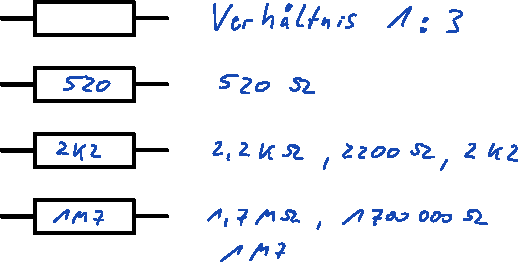
\includegraphics[width=0.3\textwidth]{images/Skizze/15_Schaltzeichen_Widerstand_Skizze.pdf}
\caption{Schaltzeichen Widerstand}
%\label{fig:}%% anpassen
\end{figure}

\begin{figure}[!ht]% hier: !ht
\centering
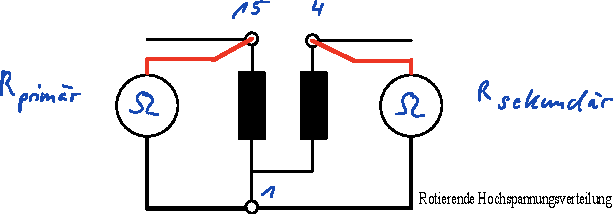
\includegraphics[width=0.6\textwidth]{images/Skizze/16_Widerstandsmessung_Skizze.pdf}
\caption{Widerstandsmessung}
%\label{fig:}%% anpassen
\end{figure}

\textbf{Messen}

Das Widerstandsmessgerät wird parallel zum Messobjekt geschaltet.

\emph{Messvoraussetzung}:

Das Messobjekt muss aus dem Stromkreis heraus gelöst sein und sich im
spannungsfreien Zustand befinden.

\textbf{Einsatzmöglichkeiten von Widerständen}

\emph{Reihe}

\begin{enumerate}
\def\labelenumi{(\arabic{enumi})}
\item
  Strombegrenzung
\item
  Spannungsteilung
\end{enumerate}

\emph{Parallel}

\begin{enumerate}
\def\labelenumi{(\arabic{enumi})}
\item
  Stromflusserhöhung
\item
  Leistungsteilung $\boxed{R_{ges} = \frac{R_{Teil}}{n}}$ (z. B.
  $n = 2 \to$ Leistung halbieren)
\end{enumerate}

\begin{figure}[!ht]% hier: !ht
\centering
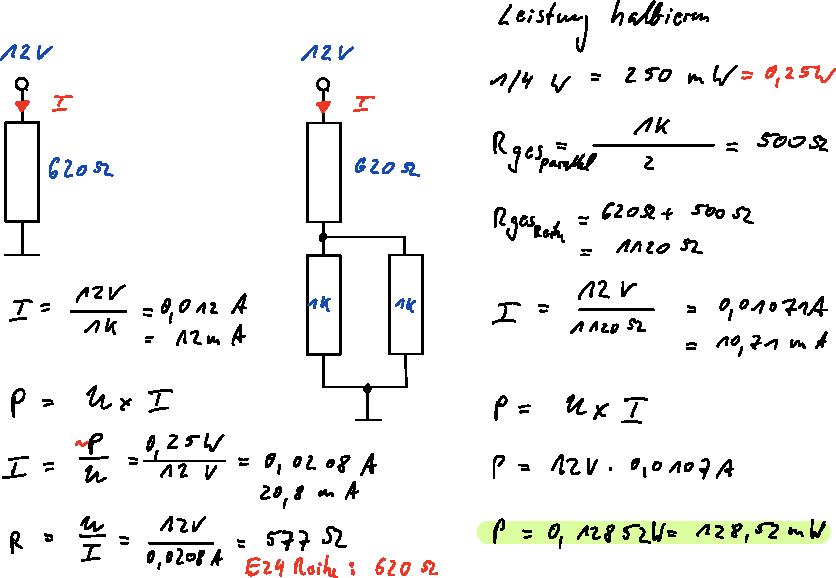
\includegraphics[width=0.6\textwidth]{images/Skizze/17_Leistungsteilung_Skizze.pdf}
\caption{Leistungsteilung}
%\label{fig:}%% anpassen
\end{figure}

\begin{figure}[!ht]% hier: !ht
\centering
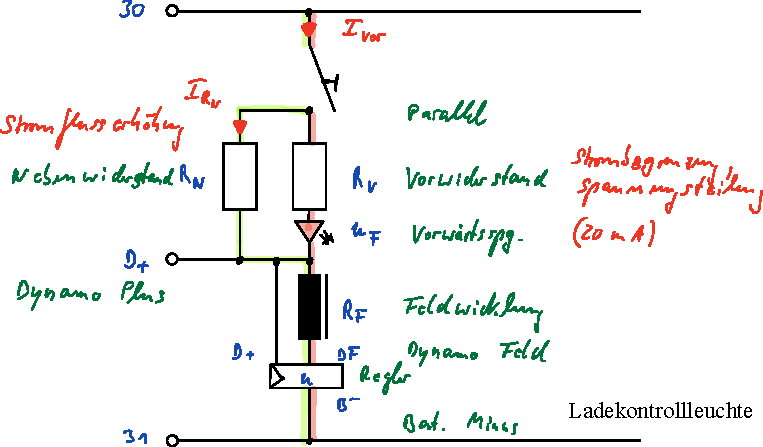
\includegraphics[width=0.6\textwidth]{images/Skizze/18_Stromflusserhoehung_Strombegrenzung_Spannungsteilung_Skizze.pdf}
\caption{Stromflusserhöhung, -begrenzung, Spannungsteilung}
%\label{fig:}%% anpassen
\end{figure}

\newpage

\section{Stromflussrichtungen}\label{stromflussrichtungen}

\begin{figure}[!ht]% hier: !ht
\centering
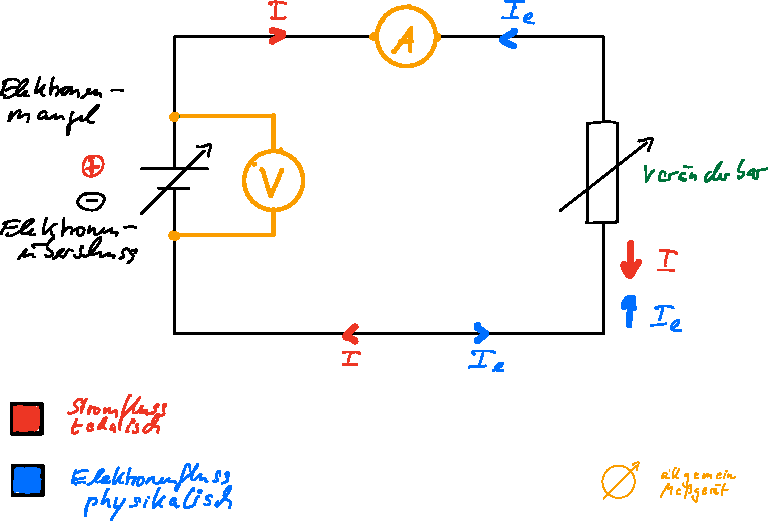
\includegraphics[width=0.6\textwidth]{images/Skizze/06_Stromfluss_Messen_Skizze.pdf}
\caption{Stromfluss und Messen}
%\label{fig:}%% anpassen
\end{figure}

\textbf{Technische Stromflussrichtung} der Strom fließt von plus nach
minus

\textbf{physikalische Stromflussrichtung} tatsächlicher Elektronenfluss,
die Elektronen bewegen sich von minus nach plus

\newpage

\section{Normgerechte Darstellung des Stromflusses durch einen
Leiter}\label{normgerechte-darstellung-des-stromflusses-durch-einen-leiter}

$\otimes$ Strom fließt vom Betrachter weg

$\odot$ Strom fließt auf den Betrachter zu

\section{Magnetfeld eines stromdurchflossenen
Leiters}\label{magnetfeld-eines-stromdurchflossenen-leiters}

Magnetfeldrichtung festlegen

\begin{figure}[!ht]% hier: !ht
\centering
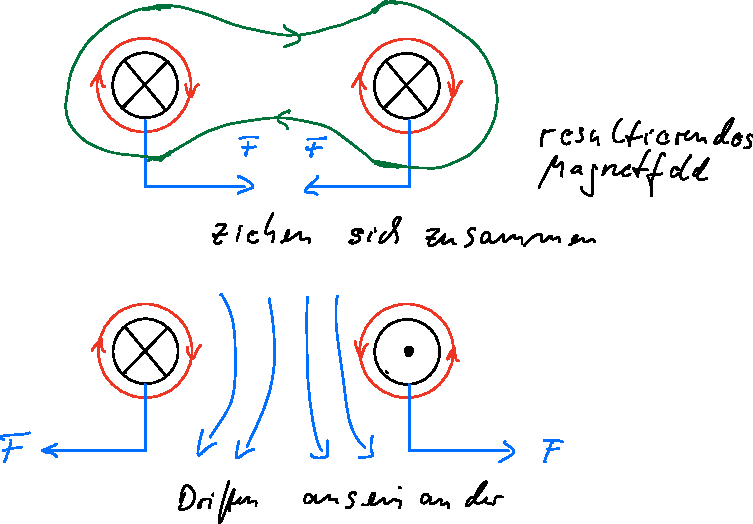
\includegraphics[width=0.6\textwidth]{images/Skizze/05_StromdurchflossenerLeiter_Skizze.pdf}
\caption{Stromdurchflossener Leiter}
%\label{fig:}%% anpassen
\end{figure}

\section{Normgerechte Festlegung des Nordpols einer stromdurchflossenen
Spule}\label{normgerechte-festlegung-des-nordpols-einer-stromdurchflossenen-spule}

\begin{figure}[!ht]% hier: !ht
\centering
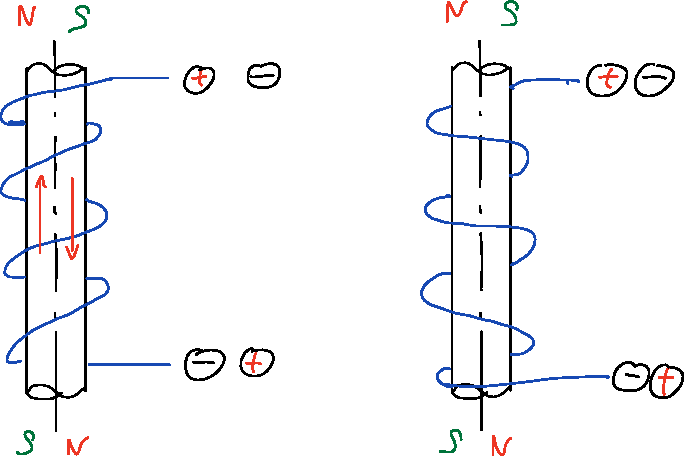
\includegraphics[width=0.6\textwidth]{images/Skizze/03_StromdurchflosseneSpule_Skizze.pdf}
\caption{Stromdurchflossene Spule}
%\label{fig:}%% anpassen
\end{figure}

Umfasst man mit der rechten Hand eine stromdurchflossene Spule so, dass
die Finger in Stromflussrichtung zeigen (technische Stromflussrichtung),
so zeigt der abgespreizte Daumen in Richtung des Nordpols.

\newpage

\section{Rechte Hand-Regel
(Generatorregel)}\label{rechte-hand-regel-generatorregel}

\begin{figure}[!ht]% hier: !ht
\centering
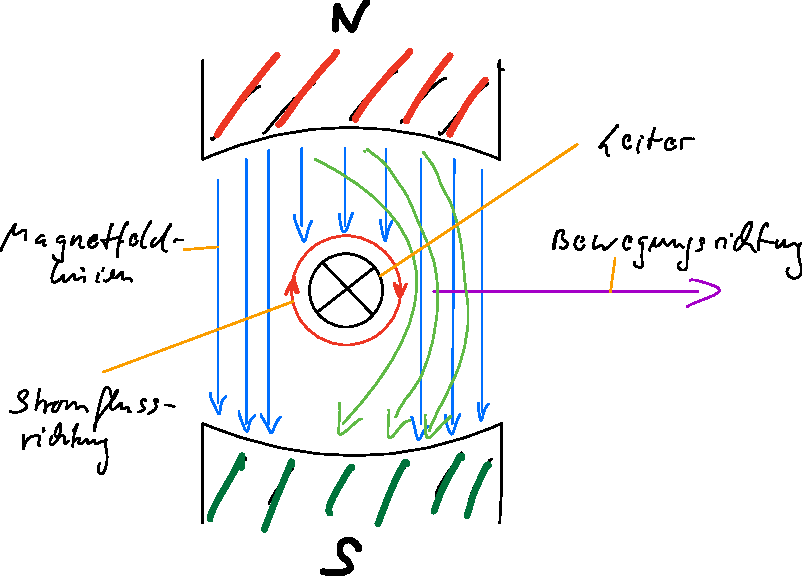
\includegraphics[width=0.6\textwidth]{images/Skizze/01_Generatorregel_Skizze.pdf}
\caption{Generatorregel}
%\label{fig:}%% anpassen
\end{figure}

Hält man die rechte Hand so in ein Magnetfeld, sodass der Nordpol in die
Handinnenfläche eintrifft. Und übt man dabei eine Bewegung in Richtung
des abgespreizten Daumens aus, so fließt ein Strom in Richtung der
Fingerspitzen.

\section{Linke Hand Regel
(Motorregel)}\label{linke-hand-regel-motorregel}

\begin{figure}[!ht]% hier: !ht
\centering
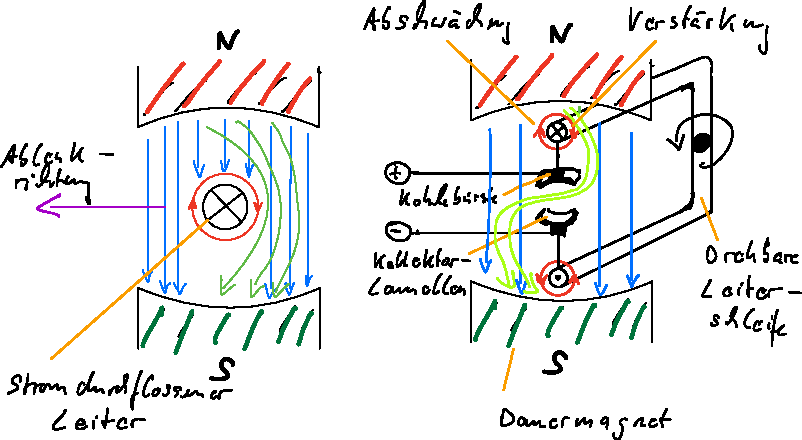
\includegraphics[width=0.6\textwidth]{images/Skizze/02_Motorregel_Skizze.pdf}
\caption{Motorregel}
%\label{fig:}%% anpassen
\end{figure}

Hält man die linke Hand so in ein Magnetfeld, dass der Nordpol in die
Handinnenfläche eintrifft und fließt dabei ein Strom in Richtung der
Fingerspitzen, so wird der Leiter in Richtung des abgespreizten Daumens
aus dem Magnetfeld abgelenkt.

\section{Das ohmsche Gesetz}\label{das-ohmsche-gesetz}

Im ohmschen Widerstand sind die Beziehungen zwischen Strom, Spannung und
Widerstand im Stromkreis festgelegt. Die Stromstärke steigt mit
zunehmender Spannung und sinkt mit zunehmendem Widerstand.

$\boxed{I = \frac{U}{R}} \quad \bigl[\frac{V}{\Omega}\bigl] = A \quad  \boxed{R = \frac{U}{I}} \quad \bigl[\frac{V}{A}\bigl] = \Omega \quad  \boxed{U = R \cdot I} \quad [\Omega \cdot A] = V$

\newpage

\section{Stromdichte J}\label{stromdichte-j}

\begin{figure}[!ht]% hier: !ht
\centering
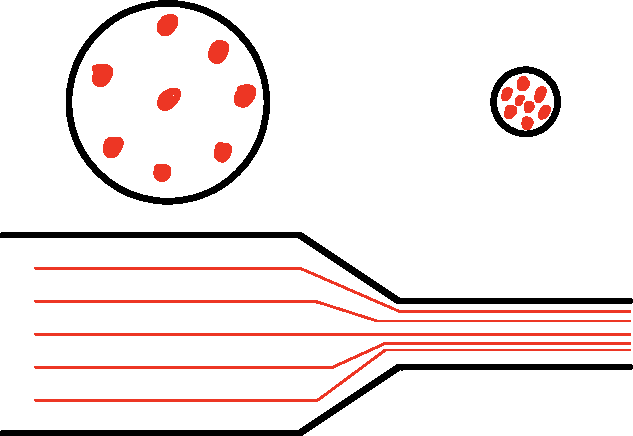
\includegraphics[width=0.4\textwidth]{images/Skizze/04_Stromdichte_Skizze.pdf}
\caption{Stromdichte}
%\label{fig:}%% anpassen
\end{figure}

\begin{itemize}
\item
  \textbf{Große Fläche}

  \begin{itemize}
  \item
    Kleine Stromdichte
  \end{itemize}
\item
  \textbf{Kleine Fläche}

  \begin{itemize}
  \item
    Große Stromdichte
  \end{itemize}
\end{itemize}

Unter Stromdichte versteht man die Anzahl der Ladungsträger Elektronen
pro Flächeninhalt $mm^2$ . Die Stromdichte ist die Ursache der
Erwärmung eines leitenden Stoffes. Ist die zu groß, wird oder kann der
Leiter zerstört werden.

\textbf{Erlaubte Stromdichte Werte:}

$J_{\text{zulässig}} = 10~\frac{A}{mm^2} \,\text{bei Kurzzeitbelastung}$

$J_{\text{zulässig}} = 30~\frac{A}{mm^2} \,\text{zugelassen (Starter)}$

\textbf{Formel}

$\boxed{J = \frac{I}{A}} \quad \bigl[\frac{A}{mm^2}\bigl] \quad  \boxed{I = J \cdot A} \quad \bigl[\frac{A \cdot mm^2}{mm^2} = A\bigl] \quad  \boxed{A = \frac{I}{J}} \quad \bigl[\frac{A \cdot mm^2}{A} = mm^2\bigl]$

\section{Leitwert G}\label{leitwert-g}

Der Leitwert ist das Vermögen eines Widerstandes einen Strom fließen
lassen zu können. Ein >>hochohmiger Widerstand<< lässt einen kleinen
Stromfluss zu. Der besitzt also einen kleinen Leitwert. Und umgekehrt
ein >>niederohmiger Widerstand<<, lässt einen hohen Stromfluss zu. Der
besitzt einen großen Leitwert. Der Leitwert ist der Kehrwert des
Widerstandes.

\textbf{Formel}

$\boxed{G = \frac{1}{R}} \quad \bigl[\frac{1}{\Omega} = S\bigl] \,\text{Siemens} \quad \boxed{R = \frac{1}{G}} \quad \bigl[\frac{1}{S} = \Omega\bigl]$

\section{Leiterwiderstand}\label{leiterwiderstand}

\emph{Abhängig}

\begin{enumerate}
\item
  Leiterlänge $l~[m] \quad R_l \sim l$
\item
  Leiterfläche $A~[mm^2] \quad R_l \sim \frac{1}{A}$
\item
  Werkstoff - spezifische Widerstand
  $\rho~\text{(rho)}~\bigl[\frac{\Omega \cdot mm^2}{m}\bigl] \quad R_l \sim \rho$
\end{enumerate}

\emph{Aluminium} $\rho_{Al} = 0,0278~\frac{\Omega \cdot mm^2}{m}$ ist
hochohmiger als \emph{Kupfer}
$\rho_{cu} = 0,0178~\frac{\Omega \cdot mm^2}{m}$.

\textbf{Leiterwiderstand R}

Er hängt von der Leiterlänge, vom spezifischen Widerstand und dem
Leiterquerschnitt ab.

\textbf{Spezifische Widerstand $\rho$ (rho)}

Ist der Widerstand eines Leiters von $1~m$ Länge und $1~mm^2$
Querschnitt.

\textbf{Formel}

$\boxed{R_l = \frac{\rho \cdot l}{A}} \, \bigl[\frac{\Omega \cdot mm^2 \cdot m}{m \cdot mm^2} = \Omega\bigl] \boxed{A = \frac{\rho \cdot l}{R_l}} \, \bigl[\frac{\Omega \cdot mm^2 \cdot m}{m \cdot \Omega} = mm^2\bigl] \boxed{l = \frac{R_l \cdot A}{\rho}} \, \bigl[\frac{\Omega \cdot mm^2 \cdot m}{\Omega \cdot mm^2} = m\bigl]$

\newpage

\section{Reihenschaltung von
Widerständen}\label{reihenschaltung-von-widerstaenden}

\begin{figure}[!ht]% hier: !ht
\centering
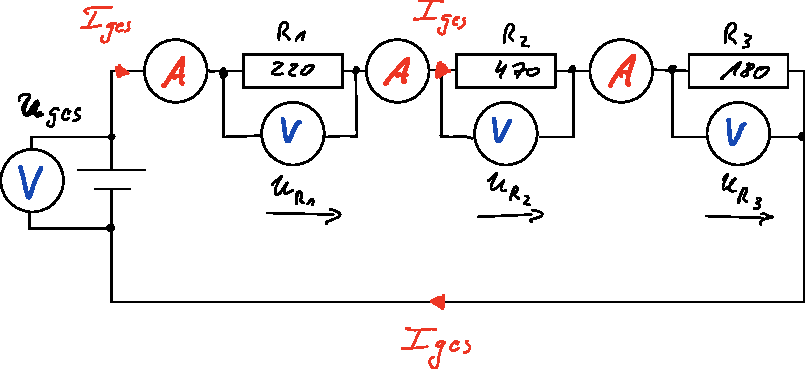
\includegraphics[width=0.6\textwidth]{images/Skizze/07_Reihenschaltung_Widerstaende_Skizze.pdf}
\caption{Reihenschaltung - Widerstände}
%\label{fig:}%% anpassen
\end{figure}

$\boxed{U = R \cdot I}$

Werden mehrere verschieden - große oder gleich große Widerstände in
Reihe geschaltet, so fällt an jedem Widerstand nach Größe des
Widerstands eine Spannung ab, die addiert die Gesamtspannung ergibt.

$\boxed{U_{ges} = U_{R_1} + U_{R_2} + U_{R_3} + \dots + U_{R_n}} \quad \bigl[V + V + V\bigl] = V$

Möchte man den Spannungsabfall an gleich großen in Reihe geschalteten
Widerständen berechnen, kann nachfolgende Gleichung verwendet werden.

$\boxed{U_{teil} = \frac{U_{ges}}{n}} \quad \bigl[\frac{V}{1}\bigl] = V$

Die Stromstärke ist an jedem Punkt des Stromkreises gleich groß, d.h.
durch jeden Widerstand fließt die gleiche Stromstärke.

$\boxed{I_{ges} = I_{R_1} = I_{R_2} = I_{R_3} = \dots = I_{R_n}} \quad \bigl[A = A = A\bigl] = A$

Der Gesamtwiderstand der Schaltung setzt sich aus der Addition der
Teilwiderstände zusammen.

$\boxed{R_{ges} = R_1 + R_2 + R_3 + \dots + R_n} \quad \bigl[\Omega + \Omega + \Omega\bigl] = \Omega$

\textbf{Rechenbeispiel}

geg:

$U_{ges} = 13,8~V$

$R_1 = 220~\Omega, R_2 = 470~\Omega, R_3 = 180~\Omega$

ges: $R_{ges}, I, U_1, U_2, U_3$

Formel

$R_{ges} = R_1 + R_2 + R_3$

$I = \frac{U_{ges}}{R_{ges}}$

$U_1 = R_1 \cdot I, U_2 = R_2 \cdot I, U_3 = R_3 \cdot I$

Lösung:

$R_{ges} = 870~\Omega$

$I = 0,0159~A$

$U_1 = 3,4897~V, U_2 = 7,4552~V, U_3 = 2,8552~V$

\newpage

\section{Relais}\label{relais}

\textbf{Arten}

\begin{enumerate}
\item
  Spannungsrelais (Schließer, Öffner, Wechsler)
\item
  Stromrelais
\end{enumerate}

\textbf{Aufgaben}

\begin{enumerate}
\item
  kleiner Spannungsabfall
\item
  kein Einfluss auf Verbraucher
\end{enumerate}

\subsection{Spannungsrelais}\label{spannungsrelais}

\begin{figure}[!ht]% hier: !ht
\centering
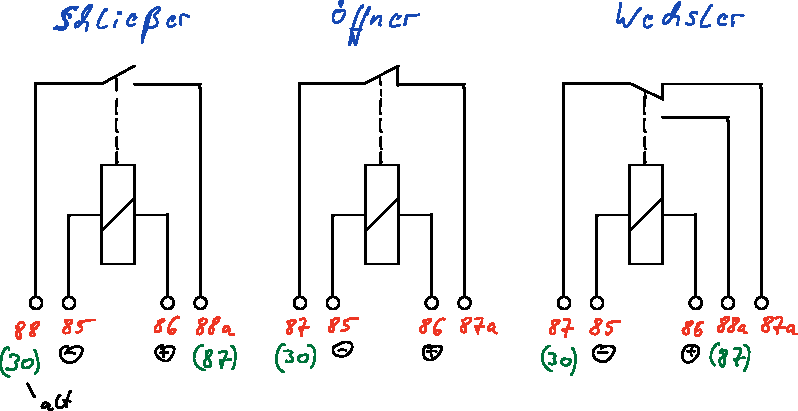
\includegraphics[width=0.7\textwidth]{images/Skizze/08_Relais_Skizze.pdf}
\caption{Relais}
%\label{fig:}%% anpassen
\end{figure}

\textbf{Ströme einer Relaisschaltung}

\begin{figure}[!ht]% hier: !ht
\centering
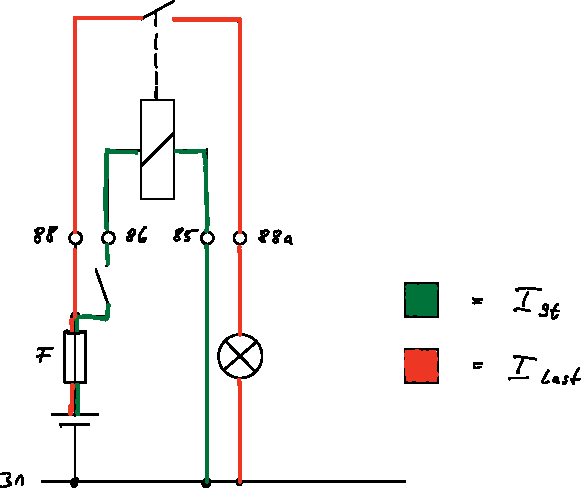
\includegraphics[width=0.4\textwidth]{images/Skizze/09_Stroeme_einer_Relaisschaltung_Skizze.pdf}
\caption{Ströme einer Relaisschaltung}
%\label{fig:}%% anpassen
\end{figure}

\begin{itemize}
\item
  \emph{Steuerstrom:} $50 - 200~mA$
\item
  \emph{Laststrom:} nach Verbraucher und Hersteller
\item
  \emph{Relaisspulenwiderstand:} $50 - 100~\Omega$ (ohne
  Schutzbeschaltung)
\end{itemize}

\subsection{Stromrelais}\label{stromrelais}

Anhängerdose Tabellenbuch (\textcite{bell:2021:tabellenbuchKfz} S. 281)

\textbf{Schaltung einer Nebelschlussleuchte bei Anhängerbetrieb}

\textbf{Schaltung mit Anhänger}

\begin{figure}[!ht]% hier: !ht
\centering
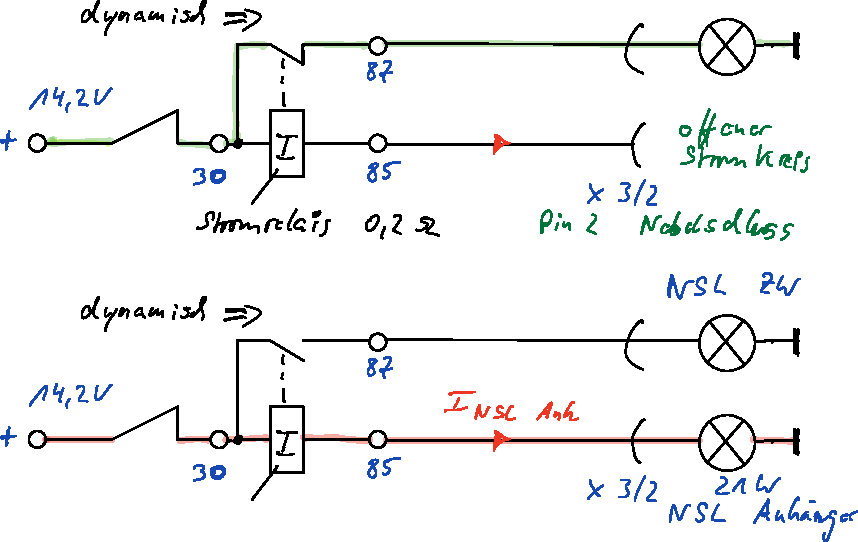
\includegraphics[width=0.6\textwidth]{images/Skizze/10_Stromrelais_Skizze.pdf}
\caption{Stromrelais}
%\label{fig:}%% anpassen
\end{figure}

\textbf{Rechenbeispiel}

geg:

$R_{Sp} = 0,2~\Omega, R_{La} = 6,85~\Omega$

$U_{ges} = 14,2~V$

ges: $R_{ges}, I, U_{K_{Sp}}, U_{K_{La}}, P$

Formel

$R_{ges} = R_{Sp} + R_{La}$

$I = \frac{U_{ges}}{R_{ges}}$

$U_{K_{Sp}} = R_{Sp} \cdot I, U_{K_{La}} = R_{La} \cdot I$

$P = U_{K_{La}} \cdot I$

Lösung:

$R_{ges} = 7,05~\Omega$

$I = 2,0142~A$

$U_{K_{Sp}} = 0,4028~V, U_{K_{La}} = 13,7972~V$

$P = 7,79~W$

\subsection{Reedkontaktschalter,
Reedrelais}\label{reedkontaktschalter-reedrelais}

Schaltzeichen Fachbuch (\textcite{brand:2020:fachkundeKfz} S. 681)

\begin{figure}[!ht]% hier: !ht
\centering
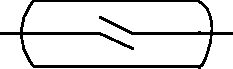
\includegraphics[width=0.1\textwidth]{images/Skizze/12_Reedkontaktschalter_Skizze.pdf}
\caption{Reedkontaktschalter}
%\label{fig:}%% anpassen
\end{figure}

\textbf{Einsatzmöglichkeiten}

\begin{enumerate}
\item
  Füllstandsanzeige

  \begin{itemize}
  \item
    Wischwasser
  \item
    Kühlwasser
  \end{itemize}
\item
  Glühkerzenausfallkontrolle
\item
  Geschwindigkeitssensor
\end{enumerate}

\subsection{Schrittrelais, Stromstoßrelais
(Stromsparen)}\label{schrittrelais-stromstossrelais-stromsparen}

\begin{figure}[!ht]% hier: !ht
\centering
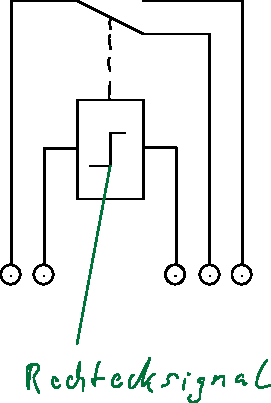
\includegraphics[width=0.15\textwidth]{images/Skizze/11_Schrittrelais_Skizze.pdf}
\caption{Schrittrelais}
%\label{fig:}%% anpassen
\end{figure}

keine Prüfung

bistabiles Relais (BMW)

\newpage

\section{Spannungsverlust - Spannungsfall - Spannungsabfall
(Prüfung)}\label{spannungsverlust-spannungsfall-spannungsabfall-pruefung}

$U_v = u$

Nennquerschnitt Tabellenbuch (\textcite{bell:2021:tabellenbuchKfz} S. 280)

Klemmbezeichnung Tabellenbuch (\textcite{bell:2021:tabellenbuchKfz} S. 273)

Spannungsfall Tabellenbuch (\textcite{bell:2021:tabellenbuchKfz} S. 280)

\begin{figure}[!ht]% hier: !ht
\centering
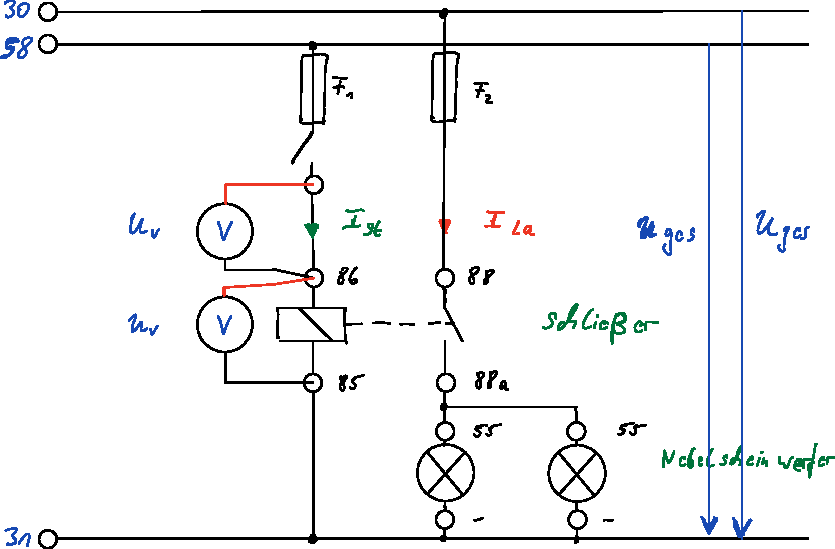
\includegraphics[width=0.65\textwidth]{images/Skizze/13_Spannungsverlust_Skizze.pdf}
\caption{Spannungsverlust}
%\label{fig:}%% anpassen
\end{figure}

\begin{table}[!ht]% hier: !ht 
\centering 
	\caption{}% \label{tab:}%% anpassen 
\begin{tabular}{@{}lll@{}}
\hline
\textbf{Bezeichnung} & \textbf{Benennung} & \textbf{Einheit} \\
\hline
$U_{ges}$ & Gesamtspannung & $[V]$ \\
$U_v$ & Spannungsverlust & $[V]$ \\
$U_k$ & Klemmspannung & $[V]$ \\
$R_l$ & Leiterwiderstand & $[\Omega]$ \\
$I$ & Stromfluss, Stromstärke & $[A]$ \\
\hline
\end{tabular} 
\end{table}

$U_{ges} = U_v + U_k;\, U_k = U_{ges} - U_v;\, U_v = U_{ges} - U_k$

$U_v = R_l \cdot I; R_l = \frac{\rho \cdot l}{A} \quad \bigl[\frac{\Omega \cdot mm^2 \cdot m}{m \cdot mm^2}\bigl] = \Omega$

$U_k = U_{ges} - R_l \cdot I$

$\boxed{U_v = \frac{\rho \cdot l \cdot I}{A}} \quad \bigl[\frac{\Omega \cdot mm^2 \cdot m \cdot A}{m \cdot mm^2}\bigl] = V$

$U_{v_{~\%}} = \frac{U_v \cdot 100}{U_{ges}} \quad \bigl[\frac{V \cdot ~\%}{V}\bigl] = ~\%$

$\boxed{U_{v_{max}} = 0,5~V}$

$\boxed{\text{max. Leiterwiderstand} = 1~\Omega}$ (außer
Starterhauptleitung)

\textbf{Spannungsfall} $U_v$ in einem stromdurchflossenen Leiter
entsteht infolge des Leiterwiderstandes ein Spannungsfall, der sich am
Verbraucher als Verlust auswirkt.

\textbf{Leiterquerschnitt} $A$ der Mindestquerschnitt einer Leitung
richtet sich nach der Stromstärke, der Leiterlänge, dem spezifischen
Widerstand des Leitermaterials und dem zulässigen Spannungsfall. Wegen
der Erwärmung des Leiters muss gegebenenfalls die Stromdichte
nachgeprüft werden.

\newpage

\section{Innenwiderstand von
Spannungsquellen}\label{innenwiderstand-von-spannungsquellen}

\begin{figure}[!ht]% hier: !ht
\centering
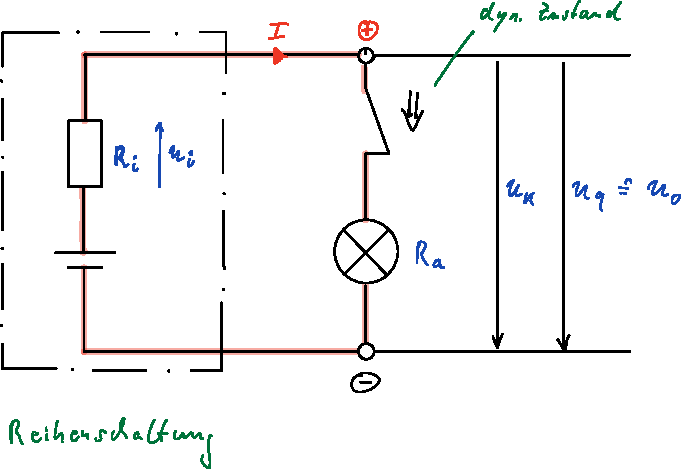
\includegraphics[width=0.6\textwidth]{images/Skizze/14_ Innenwiderstand_von_Spannungsquellen_Skizze.pdf}
\caption{Innenwiderstand von Spannungsquellen}
%\label{fig:}%% anpassen
\end{figure}

\begin{table}[!ht]% hier: !ht 
\centering 
	\caption{}% \label{tab:}%% anpassen 
\begin{tabular}{@{}lll@{}}
\hline
\textbf{Bezeichnung} & \textbf{Benennung} & \textbf{Einheit} \\
\hline
$U_q$ & Quellspannung & $[V]$ \\
$U_0 (U_{Null})$ & Leerlaufspannung & $[V]$ \\
$U_k$ & Klemmenspannung (Last, mit Verbraucher) & $[V]$ \\
$U_i$ & Spannungsabfall am Innenwiderstand & $[V]$ \\
$R_i$ & Innenwiderstand & $[\Omega]$ \\
$R_a$ & Außenwiderstand & $[\Omega]$ \\
$I$ & Stromfluss, -stärke & $[A]$ \\
\hline
\end{tabular} 
\end{table}

\textbf{Innenwiderstand} $R_i$ ist die Summe der Innenwiderstände der
Zellen. Er ist u. a. von der Temperatur und dem Lade- beziehungsweise
Entladezustand abhängig. Die Klemmenspannung $U_k$ der belasteten
Batterie ist deshalb um den Spannungsfall niedriger als die
Leerlaufspannung $U_0$.

$U_q = U_k + U_i \quad [V + V] = V$

$U_k = U_q - U_i \quad [V - V] = V$

$U_i = U_q - U_k \quad [V - V] = V$

$U_i = I \cdot R_i \quad [A \cdot \Omega] = V$

$U_k = I \cdot R_a \quad [A \cdot \Omega] = V$

$I = \frac{U_i}{R_i} \quad [\frac{V}{\Omega}] = A$

$I = \frac{U_k}{R_a} \quad [\frac{V}{\Omega}] = A$

$I = \frac{U_q}{R_{ges}} \quad [\frac{V}{\Omega}] = A$

$I = \frac{U_q}{R_i + R_a} \quad [\frac{V}{\Omega + \Omega}] = A$

$\boxed{U_k = U_q - I \cdot R_i} \quad [V - A \cdot \Omega \rightarrow V - V] = V$

$\boxed{R_i = \frac{U_i}{I}} \quad [\frac{V}{A}] = \Omega$

\textbf{Rechenbeispiel}

geg:

$U_q = 12~V, U_k = 9,6~V$

$R_a = 2,618~\Omega$ (Außenwiderstand)

ges: $I, R_i$

Formel:

$I = \frac{U_k}{R_a}$

$R_i = \frac{U_{R_i}}{I} \to R_i = \frac{(U_q - U_k)}{I}$

Lösung:

$I = 3,6669~A$

$R_i = 0,6545~\Omega$

\newpage

\section{Parallelschaltung von
Widerständen}\label{parallelschaltung-von-widerstaenden}

\begin{figure}[!ht]% hier: !ht
\centering
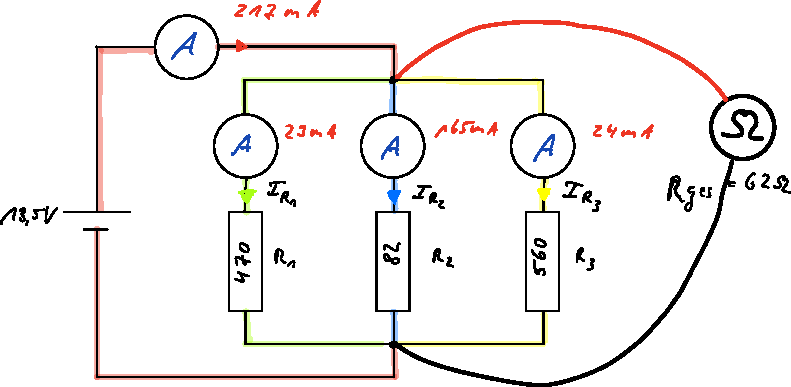
\includegraphics[width=0.6\textwidth]{images/Skizze/19_Parallelschaltung_Widerstaende_Skizze.pdf}
\caption{Parallelschaltung von Widerstände}
%\label{fig:}%% anpassen
\end{figure}

Werden mehrere verschiedene - oder gleich große Widerstände parallel
geschaltet, so fließt durch jeden Widerstand, nach Größe des
Widerstandes ein Strom, der addiert den Gesamtstrom ergibt.

$I_{ges} = I_{R_1} + I_{R_2} + I_{R_3} + \dots + I_{R_n} \quad [A + A + A] = A$

An jeden parallel geschalteten Widerstand liegt die gleiche Spannung an.

$U_{ges} = U_{R_1} = U_{R_2} = U_{R_3} = \dots = U_{R_n} \quad [V = V = V] = V$

Der Gesamtwiderstand ist stets kleiner als der kleinste
Einzelwiderstand.

$R_{ges} = \frac{1}{\frac{1}{R_1} + \frac{1}{R_2} + \frac{1}{R_3} + \dots + \frac{1}{R_n}} \quad \bigl[\frac{1}{\frac{1}{\Omega} + \frac{1}{\Omega} + \frac{1}{\Omega}} = \frac{1}{\frac{1}{\Omega}} = \frac{1}{S}\bigl] = \Omega$

Möchte Mann/Frau den Gesamtwiderstand von gleich großen parallel
geschalteten Widerständen berechnen, kann nachfolgende Gleichung
angewendet werden.

$R_{ges} = \frac{R_{Teil}}{n} \quad \bigl[\frac{\Omega}{1}\bigl] = \Omega \quad \to n = \frac{R_{Teil}}{R_{ges}} \quad \bigl[\frac{\Omega}{\Omega}\bigl] = 1$

n = Anzahl der Widerstände (gleich große Widerstände)

$R_{ges} = \frac{R_1 \cdot R_2}{R_1 + R_2}$

$R_{ges} = \frac{1}{\frac{1}{R_1} + \frac{1}{R_2} + \frac{1}{R_3}}$

$\to R_{1} = \frac{1}{\frac{1}{R_{ges}} - \frac{1}{R_2} - \frac{1}{R_3}} \quad \to R_{2} = \frac{1}{\frac{1}{R_{ges}} - \frac{1}{R_1} - \frac{1}{R_3}} \quad \to R_{3} = \frac{1}{\frac{1}{R_{ges}} - \frac{1}{R_1} - \frac{1}{R_2}}$

\textbf{Rechenbeispiel}

geg: \textbar\textbar{}

$U = 13,5~V$ (Hinweis: $U_{ges} = U$)

$R_1 = 470~\Omega, R_2 = 82~\Omega, R_3 = 560~\Omega$

ges: $I_{ges}, I_1, I_2, I_3, R_{ges}$

Formel:

$I_1 = \frac{U}{R_1}, I_2 = \frac{U}{R_2}, I_3 = \frac{U}{R_3}$

$I_{ges} = I_1 + I_2 + I_3$

$R_{ges} = \frac{U}{I_{ges}}$

Lösung:

$I_1 = 0,0287~A, I_2 = 0,1646~A, I_3 = 0,0241~A$

$I_{ges} = 0,2175~A$

$R_{ges} = 62,079~\Omega$

\newpage

\section{gemischte Schaltung}\label{gemischte-schaltung}

\begin{figure}[!ht]% hier: !ht
\centering
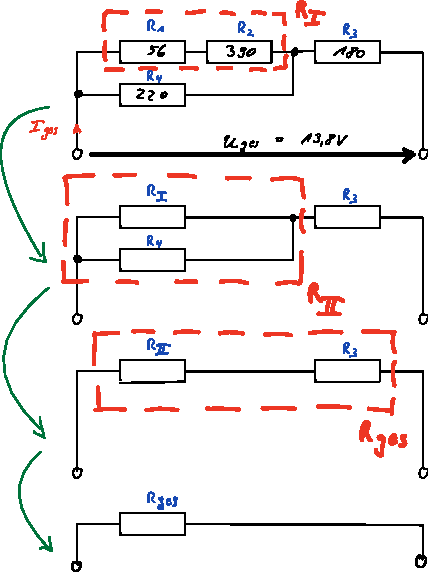
\includegraphics[width=0.6\textwidth]{images/Skizze/25_gemischte_Schaltung.pdf}
\caption{gemischte Schaltung}
%\label{fig:}%% anpassen
\end{figure}

$R_\mathrm{I} = R_1 + R_2$

$R_\mathrm{II} = \frac{1}{\frac{1}{R_\mathrm{I}} + \frac{1}{R_4}}$

$R_{ges} = R_\mathrm{II} + R_3$

Gemischte Schaltungen berechnet man, indem man sie in Reihen- und
Parallelschaltungen zerlegt und Ersatzwiderstände bildet.

\textbf{Rechenbeispiel}

geg:

$R_1 = 56~\Omega, R_2 = 390~\Omega, R_3 = 180~\Omega, R_4 = 220~\Omega$

$U_{ges} = 13,8~V$

ges: $U_{Teil}, R_{Teil}, I_{Teil}, I_{{ges}}, R_{ges}$

Formel:

$R_I = R_1 + R_2$

$R_{II} = \frac{1}{\frac{1}{R_I} + \frac{1}{R_4}}$

$R_{ges} = R_{II} + R_3$

$I_{ges} = \frac{U_{ges}}{R_{ges}}$

$U_{R_3} = R_3 \cdot I_{ges}$

$U_{R_{II}} = R_{II} \cdot I_{ges}$

$I_{R_I} = \frac{U_{R_{II}}}{R_I}$

$I_{R_4} = \frac{U_{R_{II}}}{R_4}$

$U_{R_1} = R_1 \cdot I_{R_I}$

$U_{R_2} = R_2 \cdot I_{R_I}$

Lösung:

$R_I = 446~\Omega, R_{II} = 147,3273~\Omega$

$R_{ges} = 327,3273~\Omega$

$I_{ges} = 0,0422~A$

$U_{R_3} = 7,5887~V, U_{R_{II}} = 6,2113~V$

$I_{R_I} = 0,0139~A, I_{R_4} = 0,0282~A$

$U_{R_1} = 0,7799~V, U_{R_2} = 5,4314~V$

\newpage

\section{Die elektrische Leistung}\label{die-elektrische-leistung}

$P$ (Power) Watt, $[W], [kW]$

\emph{schottischer Ingenieur James Watt (1736-1819)}

Glühlampe $12~V/21~W$, Wärmestrahlerbeleuchtungskörper

\begin{figure}[!ht]% hier: !ht
\centering
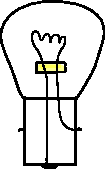
\includegraphics[width=0.12\textwidth]{images/Skizze/26_Leistung_Gluehlampe.pdf}
\caption{Leistung Glühlampe}
%\label{fig:}%% anpassen
\end{figure}

$\boxed{P = U \cdot I} \quad [V \cdot A] = W$

$\boxed{U = \frac{P}{I}} \quad [\frac{W}{A} \to \frac{V \cdot A}{A}] = V$

$\boxed{I = \frac{P}{U}} \quad [\frac{W}{V} \to \frac{V \cdot A}{V}] = A$

\textbf{wenn $I$ fehlt} (Einsetzverfahren)

$P = U \cdot I \quad [V \cdot A] = W, \quad I = \frac{U}{R} \quad [\frac{V}{\Omega}] = A$

$P = U \cdot \frac{U}{R} \to \boxed{P = \frac{U^2}{R}} \quad [\frac{V \cdot V}{\Omega} \to A \cdot V] = W$

\textbf{wenn $U$ fehlt} (Einsetzverfahren)

$P = U \cdot I \quad [V \cdot A] = W, \quad U = R \cdot I \quad [\Omega \cdot A] = V$

$P = R \cdot I \cdot I \to \boxed{P = R \cdot I^2} \quad [\Omega \cdot A \cdot A \to V \cdot A] = W$

Die elektrische Leistung $P$ ist das Produkt aus Spannung $U$ und
Strom $I$.

\textbf{Anmerkung} die verschiedenen Leistungen der unterschiedlichen
Verbraucher, in Schaltungen, addieren sich zur Gesamtleistung.

\textbf{Merke} halbe Spannung bedeutet nicht halbe Leistung und
umgekehrt halbe Leistung bedeutet nicht halbe Spannung, die Leistung
ändert sich im Quadrat.

Bei der Berechnung an/von Wärmestrahlerbeleuchtungskörpern, zuerst den
Widerstand berechnen.
 \newpage
\chapter{Verbrennungsmotor - Elektrik}
%ju 28-Mai-22 02-Verbrennungsmotor-Elektrik.tex
\section{Kraftstoffpumpenrelais}\label{kraftstoffpumpenrelais}

\textbf{Nenne 3 Abschaltmöglichkeiten. Weshalb werden überhaupt das
Kraftstoffpumpenrelais und damit die Kraftstoffförderpumpe
abgeschaltet?}

\begin{enumerate}
\item
  \textbf{Konventionelle Abschaltung durch das Steuergerät}

  Bei Abstellung des Motors wird das Kraftstoffförderpumpenrelais vom SG
  nicht mehr angesteuert, somit wird kein Kraftstoff mehr gefördert.
\item
  \textbf{Ausfall des Bezugsmarken-Drehzahlgebers}

  Fällt der \emph{Bezugsmarken-Drehzahlgeber} aus, während des Betriebs
  oder bei Stillstand des Motors, kann das SG den ersten Zylinder nicht
  mehr zuordnen. Der Motor springt nicht mehr an. Ist dieses der Fall,
  schaltet das SG das Kraftstoffförderpumpenrelais ab. Mit dem
  Abschalten werden nachfolgende Komponenten nicht mehr mit Spannung
  versorgt:

  \begin{itemize}
  \item
    Kraftstoffförderpumpe
  \item
    alle Einspritzventile
  \item
    Tankentlüftungsventil
  \item
    Lambdasondenheizung
  \end{itemize}
\item
  \textbf{Volllaufsicherung}

  Sollte der Motor durch ein unbeabsichtigtes Manöver des Fahrers einmal
  zum Stillstand gekommen sein, liefert der
  \emph{Bezugsmarken-Drehzahlgeber} kein Signal mehr, aufgrund des
  stehenden Motors, an das SG. Sobald dieses Signal ausbleibt, schaltet
  das SG das Kraftstoffpumpenrelais ab, die Kraftstoffförderpumpe
  fördert keinen Kraftstoff mehr.

  \textbf{Hintergrund}: Es kann ja sein, dass ein Einspritzventil
  undicht ist, das Einlassventil offen steht, somit würde, wenn die
  Kraftstoffförderpumpe weiterhin Kraftstoff fördert, in den
  entsprechenden Zylinder Kraftstoff eingespritzt. Er läuft also voll.
  Wird nun, nach einer Weile, wieder ein Startvorgang durchgeführt,
  kommt es zu einem kapitalen Folgeschaden, da nach dem
  \emph{Pascalschen Gesetz}, Flüssigkeiten sich nicht zusammendrücken
  lassen. Die Folge wären mechanische Defekte am Kurbeltrieb und Kolben.
\end{enumerate}

\textbf{Verunfallen}

Kommt es zu einem Unfall, mit dem Auslösen des Airbags und
anschließenden Überschlägen des Fahrzeugs, möchte man nicht, dass die
Kraftstoffförderpumpe weiterhin Kraftstoff fördert. Es ist auch möglich,
dass aus einer Kraftstoffleitung unkontrolliert Kraftstoff austritt, der
sich unweigerlich an heißen Fahrzeugteilen, oder an
Kurzschlussfunkenbildung entzünden würde.

\textbf{Wann läuft die Kraftstoffpumpe an?} $\to$ über
Türkontaktschalter

\section{Sekundärluftpumpe}\label{sekundaerluftpumpe}

Das \textbf{Sekundärluftsystem} wird bei Ottomotoren in der
Kaltstartphase (3-5 Min.) aktiviert, um die Abgasbestandteile HC und CO
in der Warmlaufphase zu minimieren, durch eine thermische
Nachverbrennung.

\textbf{Sekundärluftpumpe} Umgebungsluft anzusaugen und diese in den
Abgaskrümmer hinter den Auslassventilen einzublasen.

Durch Oxidation entsteht Wärme (unverbrannte Kohlenwasserstoffe
reagieren mit Sauerstoff, Wärmeenergie wird frei)

\emph{Ziel} 350 °C >>light-off-Point<< schnell erreichen.)

\emph{Betriebstemperatur Katalysator} 650 bis 800 °C

\section{3-Wege-Kat}\label{wege-kat}

\textbf{Welche Schadstoffe werden im Oxidationskatalysator zu welchen
Stoffen umgewandelt?}

\textbf{Aufbau Katalysator} Keramik- o. Metallträger, Zwischenschicht
(Wash-Coat, Oberfläche vergrößern), katalytisch aktive Schicht
(Edelmetalle: Rhodium, Platin)

\emph{Die chemischen Reaktionsgleichungen lauten:}

\begin{enumerate}
\item
  \textbf{Kohlenmonoxid} $CO$ + $O_2$ wird umgewandelt zu $CO_2$ =
  Kohlendioxid, Sauerstoff wird verbraucht

  \begin{itemize}
  \item
    Katalysator = Platin $\to$ Oxidationsprozess
  \end{itemize}
\item
  \textbf{unverbrannte Kohlenwasserstoffe} $HC$ + $O_2$ werden
  umgewandelt zu $CO_2$ + $H_2O$ = Kohlendioxid und Wasser,
  Sauerstoff wird verbraucht

  \begin{itemize}
  \item
    Katalysator = Platin $\to$ Oxidationsprozess
  \end{itemize}
\item
  \textbf{Stickoxide} $NO_\text{x}$ wird umgewandelt zu $N_2$ +
  $O_2$, Sauerstoff wird freigesetzt

  \begin{itemize}
  \item
    Katalysator = Rhodium $\to$ Reduktionsprozess
  \end{itemize}
\end{enumerate}

\textbf{Weshalb werden Oxidationskatalysatoren vor den Partikelfiltern
eingebaut?}

Durch den Oxidationsprozess entsteht eine höhere Abgastemperatur, diese
höhere Abgastemperatur unterstützt die Regenration des Partikelfilters,
das heißt, die Partikel können dadurch abgebrannt werden.

\section{AdBlue}\label{adblue}

\textbf{Was ist an dem Motor anders? Warum braucht der Motor AdBlue?}

\begin{itemize}
\item
  höheres Verdichtungsverhältnis $\to$ weniger Kraftstoff notwendig
\item
  höhere Wärme und Druck
\item
  mehr Stickoxide
\end{itemize}

AdBlue

\begin{itemize}
\item
  Reduktionsmittel
\item
  gefriert - 11 °C
\item
  32,5 \% ca. 1/3 Harnstoff + 2/3 demineralisiertes Wasser (rein)
\end{itemize}

\textbf{chemische Prozess AdBlue} Hydrolysestrecke Harnstoff $\to$
Ammoniak (säurehaltig) $\to$ SCR-Kat $\to$ $NO_\text{x}$ +
Ammoniak umgewandelt in Stickstoff + Wasser

\section{Wie kann ich den Einsatz von Kraftstoff reduzieren?
(Nacheinspritzung
weglassen)}\label{wie-kann-ich-den-einsatz-von-kraftstoff-reduzieren-nacheinspritzung-weglassen}

$\to$ Ausgangspunkt: Temperatur 550 °C notwendig

\textbf{Wie?}

\begin{itemize}
\item
  höherer Druck $\to$ höhere Temperatur
\item
  Ansauglufterwärmung (Kondensationsverluste reduzieren)
\item
  Glühkerzen

  \begin{itemize}
  \item
    \emph{Vorglühen} (Kaltstart)
  \item
    \emph{Zwischen glühen} (weniger Kraftstoff einsetzen)
  \end{itemize}
\end{itemize}

\section{Schubabschaltung
(Voraussetzung)}\label{schubabschaltung-voraussetzung}

\begin{enumerate}
\item
  Drosselklappen geschlossen (Leerlaufkontakt)
\item
  Kein Kraftstoff eingespritzt
\item
  Motortemperatur $>$ 80 °C
\item
  Drehzahl $>$ wieder Einsetzdrehzahl (1400-1700 U/min)
\end{enumerate}

\section{Schichtladebetrieb - homogene
Gemischbildung}\label{schichtladebetrieb-homogene-gemischbildung}

\textbf{Umschalten} erfolgt durch Gas geben: Schichtladebetrieb $\to$
homogene Gemischbildung

\textbf{Wie kann ich das klingeln vermeiden?}

$\to$ Ausgangslage Verdichtungsverhältnis bleibt konstant

$\to$ Brennraumtemperatur herabsetzen, wie?

\begin{enumerate}
\item
  \textbf{Zündzeitpunkt auf Spät verstellen,} d.h. 15° vor OT

  \begin{itemize}
  \item
    $\to$ Verbrennungshöchstdruck wird später erreicht, 20° nach OT
  \item
    Kolben wird weiter geschoben durch die vorhergehende Verbrennung
  \item
    AV öffnet 148° nach OT, wir haben ein heißeres Abgas

    \begin{itemize}
    \item
      $\to$ der Katalysator kommt schneller auf Betriebstemperatur
    \item
      Wenn der Raum größer wird, nimmt der Druck ab und damit die
      Temperatur. (Hier nicht voll ausgenutzt, und damit habe ich ein
      heißeres Abgas)
    \end{itemize}
  \item
    \textbf{weniger Leistung} wird in Kauf genommen
  \end{itemize}
\item
  \textbf{Kraftstoff Einspritzen}

  durch den Kraftstoff Einspitzen entziehe ich dem Verbrennungsprozess
  Wärme, dadurch wird die Brennraumtemperatur geringer, geringerer Druck
  und dadurch die Neigung zum Klingeln beseitigt
\end{enumerate}

\textbf{Wärmekraftmaschine}

Ottomotor / \textbf{Gleichraumverbrennung} / Kraftstoff-Luft Gemisch
verdichten reicht nicht aus um einen sehr hohen Verbrennungsdruck und
Temperatur zu bekommen, hier ist eine Zündkerze notwendig.

Vor Ende des Verdichtungstaktes 25-30° vor OT wird das komprimierte
Kraftstoff-Luftgemisch fremdgezündet über den Funken der Zündkerze.
(Entflammung)

Der Verbrennungshöchstdruck wird erreicht bei 3-6° nach OT, damit
bekommt der Kolben ein auf den Deckel und geht nach unten.

\textbf{Höheres Verdichtungsverhältnis} (Nachteil) höhere Drücke $\to$
Kurbelwellenlager

\section{Lenkrollradius}\label{lenkrollradius}

\textbf{Fahrzeug mit Lenkrollradius Null bekommen in der Regel eine
Lenkunterstützung eingebaut? (Hintergrund)}

Lenkrollradius = Lenkrollhalbmesser

\begin{figure}[!ht]% hier: !ht
\centering
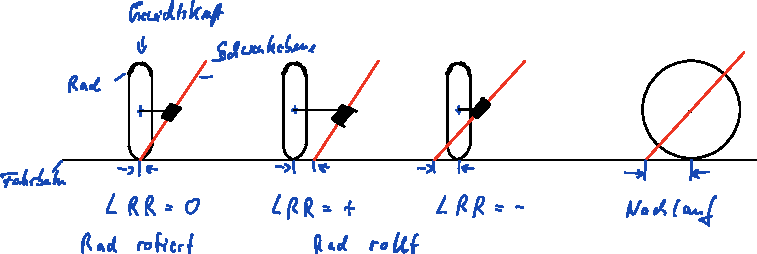
\includegraphics[width=0.6\textwidth]{images/Skizze/27_FT_Lenkrollradius_Nachlauf.pdf}
\caption{Lenkrollradius und Nachlauf}
%\label{fig:}%% anpassen
\end{figure}

Bei einem \textbf{Lenkrollhalbmesser} $0$ trifft die Verlängerung der
Lenkachse (Schwenkachse) mit der Mitte des Radaufstandspunktes in einem
Punkt auf die Fahrbahn.

Erfordert \textbf{hohe Lenkkräfte} im Stand, Rad radiert auf der Stelle,
Vorteil spurstabil.

Lenkrollhalbmesser wird bestimmt durch Sturz, Spreizung und
Einpresstiefe der Felge.

\textbf{Negativer Lenkrollhalbmesser} wird bevorzugt

\begin{itemize}
\item
  Vorteil Fahrzeug bleibt stabilisierend
\item
  Flatterneigung
\item
  Rad rollt um den Drehpunkt herum
\end{itemize}

Nachlauf (Teewagenprinzip)
 \newpage
\chapter{Grundlagen - Elektrik 2}
%ju 28-Mai-22 03-Grundlagen-Elektrik2.tex
\section{Potentialbestimmung}\label{potentialbestimmung}

\begin{figure}[!ht]% hier: !ht
\centering
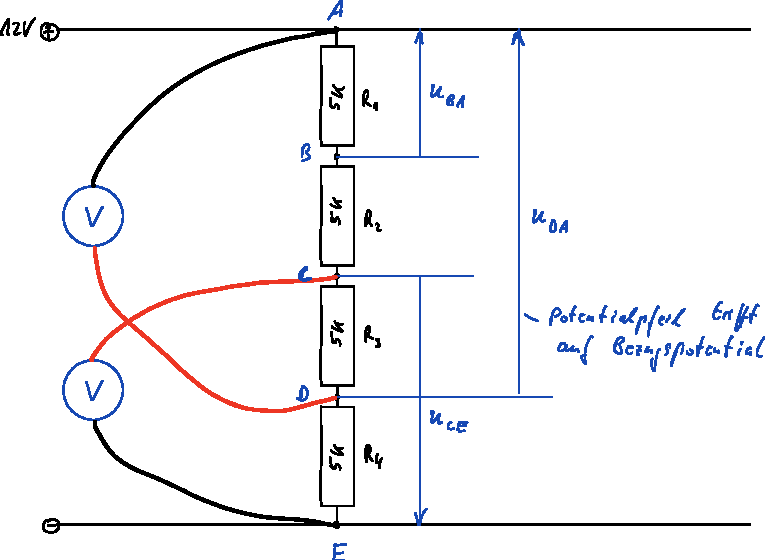
\includegraphics[width=0.6\textwidth]{images/Skizze/28_FT_Potentialbestimmung.pdf}
\caption{Potentialbestimmung}
%\label{fig:}%% anpassen
\end{figure}

Klemmenspannung und Potential

\begin{itemize}
\item
  $U_{R_1} = 3~V$, $U_{R_3} = 3~V$
\item
  $U_{CE} = 6~V$, $U_{BA} = -3~V$, $U_{DA} = -9~V$
\end{itemize}

Möchte man das/ein Potential an einem Punkt in einem Stromkreis
messen/bestimmen, bezieht man sich immer auf ein Bezugspotenzial. Die
Schreibweise dieser Messung lautet dann zum Beispiel $U_{CE}$, hierbei
möchte ich also das Potential C messen, C ist der erste Buchstabe, an
ihm wird der \emph{rote Clip} des Multimeters angeschlossen. Das
Bezugspotenzial hierbei E ist der zweite Buchstabe, hier wird
grundsätzlich der \emph{schwarze Clip} des Multimeters angeschlossen.
Potentialbestimmungen können auch zeichnerisch dargestellt werden.
Hierbei lautet die Vereinbarung, die Pfeilspitze des Spannungs- oder
Potentialpfeils trifft immer auf das Bezugspotenzial. Beispiel
$U_{DA}$.

\newpage

\section{Brückenschaltung -
Brückenspannung}\label{brueckenschaltung-brueckenspannung}

\begin{figure}[!ht]% hier: !ht
\centering
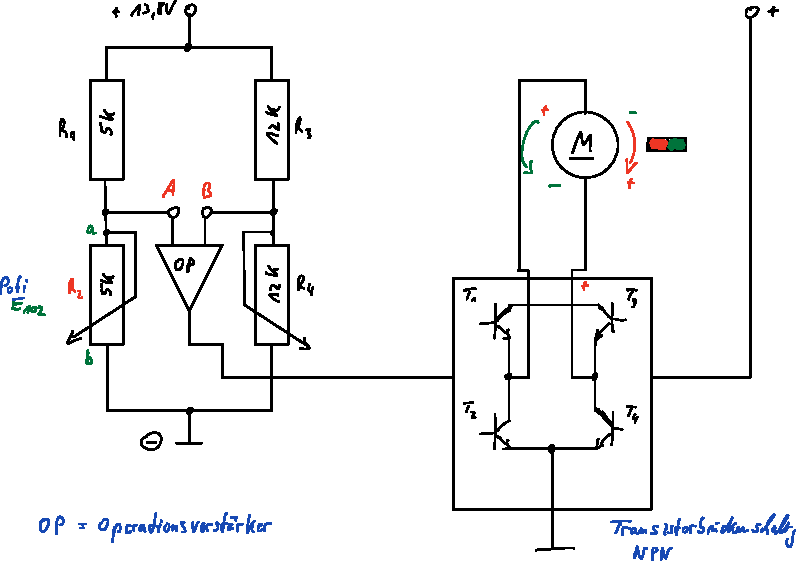
\includegraphics[width=0.6\textwidth]{images/Skizze/28_FT_Brueckenschaltung.pdf}
\caption{Brückenschaltung}
%\label{fig:}%% anpassen
\end{figure}

$U_{A\text{-}} = 6,9~V$, $U_{B\text{-}} = 6,9~V$, $U_{AB} = 0~V$
(keine Differenz)

$U_{A\text{+}} = -6,9~V$, $U_{B\text{+}} = -6,9~V$, $U_{AB} = 0~V$
(keine Differenz)

Poti $\to R_2 = 1~k$

$I_{Li} = \frac{U_{ges}}{R_{{Li}_{ges}}} = \frac{U_{ges}}{R_1 + R_2} = \frac{13,8}{5000 + 1000} =0,0023~A$

$U_{R_1} = R_1 \cdot I_{Li} = 5000~\Omega \cdot 0,0023~A = 11,5~V$

$U_{A\text{+}} = -11,5~V$, $U_{B\text{+}} = -6,9~V$,
$U_{AB} = -4,6~V$

$I_{Re} = \frac{U_{R_3}}{R_3} = \frac{11,5}{12000} =0,00096~A$

$R_4 = \frac{U_{R_4}}{I_{Re}} = \frac{U_{ges} - U_{R_3}}{I_{Re}} = \frac{13,8 - 11,5}{0,00096} = 2395,83~\Omega$

\newpage

\section{Signalanlage Oldtimer
(Prüfung)}\label{signalanlage-oldtimer-pruefung}

\textbf{Aufgabe:} Stromlaufplan zeichnen

Ein Kunde beanstandet Folgendes:

\textbf{>>Wenn ich den Fahrtrichtungsanzeiger setze und dabei das
Bremspedal betätige, bleibt mein Fahrtrichtungsanzeiger stehen.<<}

Lösen Sie dieses Problem mit einem entsprechenden Relaisschaltung.
Komponenten, die vorhanden sein müssen: Batterie, 30/15/31ger Schiene,
Blinkrelais (2-polig), Kontrollleuchte, Blinkerschalter, zwei
Blinkleuchten links, zwei Blinkleuchten rechts. Dazu ein entsprechendes
Relais.

\textbf{Problem - Spannungsverlust durch Bremse treten}

\begin{figure}[!ht]% hier: !ht
\centering
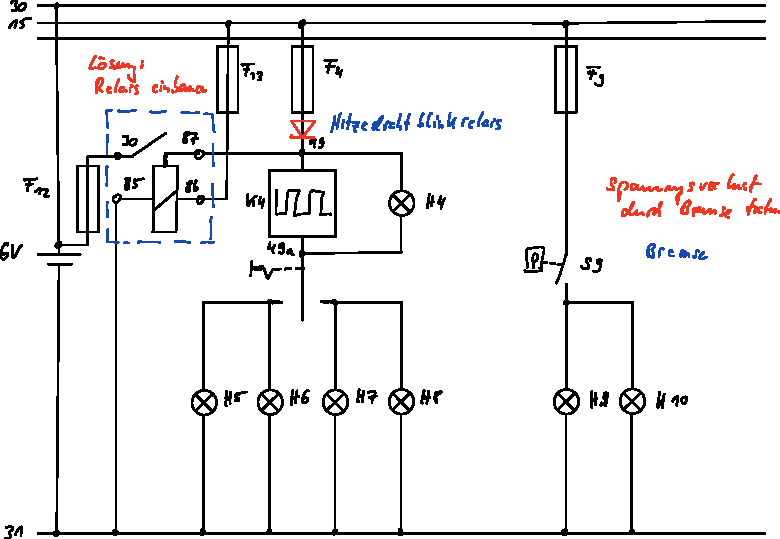
\includegraphics[width=0.9\textwidth]{images/Skizze/29_FT_Signalanlage_Relais_6V.pdf}
\caption{Signalanlage Oldtimer Relais}
%\label{fig:}%% anpassen
\end{figure}

\emph{Lösung} $\to$ Relais einbauen.

\emph{Zündung Einschalten} Steuerstrom baut magnetisches Feld auf und
schneidet die Spule, induziert dabei eine Spannung von $6~V$.

\textbf{Blinkfrequenz} $90 \pm30$ Impulse pro Minute

\emph{Zündung ausschalten} Diode einbauen zwischen F4 und Anschluß 49

\newpage

\section{Tagfahrlicht verdrahten mit Relais Öffner oder
Schließer}\label{tagfahrlicht-verdrahten-mit-relais-oeffner-oder-schliesser}

\textbf{Vorteile LED}

\begin{itemize}
\item
  Stromverbrauch
\item
  Haltbarkeit
\item
  Bezeichnung >>RL<<
\item
  Abstand $600~mm$
\end{itemize}

\begin{figure}[!ht]% hier: !ht
\centering
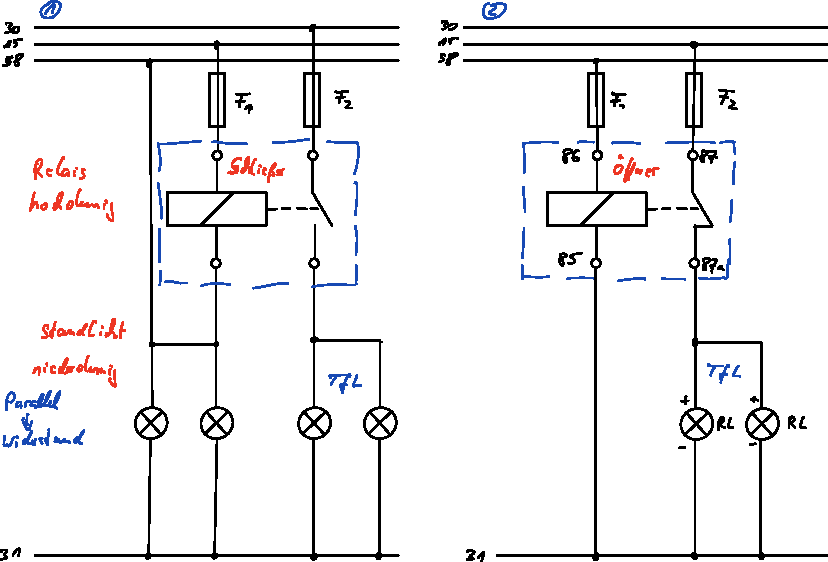
\includegraphics[width=0.9\textwidth]{images/Skizze/29_FT_Tagfahrlicht_Relais.pdf}
\caption{Tagfahrlicht Relais}
%\label{fig:}%% anpassen
\end{figure}

\textbf{1) Wieso leuchtet das Tagfahrlicht ohne Standlicht?} - Das
Relais ist hochohmig und das Standlicht (4x Lampen parallel) ist
niederohmig. - Das Relais holt sich die Masse über die Lampen.

\textbf{2) Was muss ich machen, damit ich Kraftstoff einsparen kann?} -
Vgl. Abb. Tagfahrlicht - (1) Sicherung \emph{F1} ziehen - (2) Sicherung
\emph{F1} und \emph{F2} ziehen

\newpage

\section{Elektromotorarten}\label{elektromotorarten}

\subsection{Nebenschlussmotor}\label{nebenschlussmotor}

Urmotor im Kfz, außer Starter

\begin{table}[!ht]% hier: !ht 
\centering 
	\caption{}% \label{tab:}%% anpassen 
\begin{tabular}{@{}ll@{}}
\hline
\textbf{Abk.} & \textbf{Bezeichnung} \\
\hline
$AW$ & Ankerwicklung (Spule) \\
$NSW$ & Nebenschlusswicklung (Spule) \\
$I_A$ & Ankerstrom \\
$I_{NSW}$ & Stromfluss durch die NSW \\
$RSW$ & Reihenschlusswicklung \\
$I_{RSW}$ & Stromfluss durch die RSW \\
\hline
\end{tabular} 
\end{table}

\textbf{a) Nebenschlussmotor mit Feldwicklung}

Kennlinie - Drehzahlverhalten

\begin{figure}[!ht]% hier: !ht
\centering
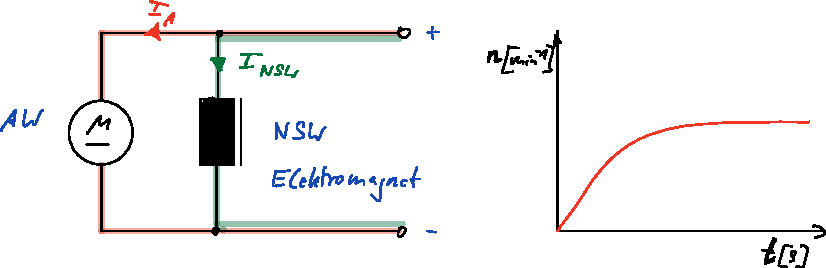
\includegraphics[width=0.6\textwidth]{images/Skizze/30_FT_Nebenschlussmotor_mit_Feldwicklung.pdf}
\caption{Nebenschlussmotor mit Feldwicklung}
%\label{fig:}%% anpassen
\end{figure}

\textbf{b) Nebenschlussmotor mit Permanenterregung}

Kennlinie - Drehzahlverhalten

\begin{figure}[!ht]% hier: !ht
\centering
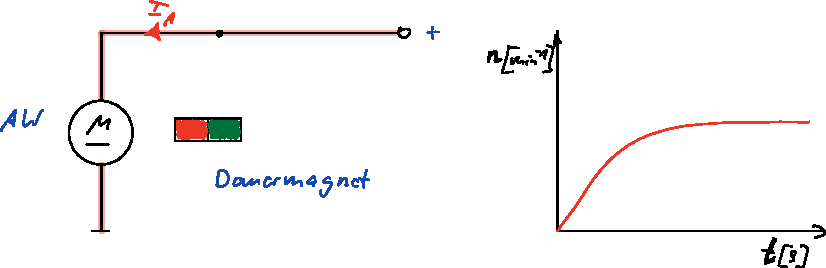
\includegraphics[width=0.6\textwidth]{images/Skizze/30_FT_Nebenschlussmotor_mit_Permanenterregung.pdf}
\caption{Nebenschlussmotor mit Permanenterregung}
%\label{fig:}%% anpassen
\end{figure}

\subsection{Reihenschlussmotor}\label{reihenschlussmotor}

Dreht hoch

Kennlinie - Drehzahlverhalten

\begin{figure}[!ht]% hier: !ht
\centering
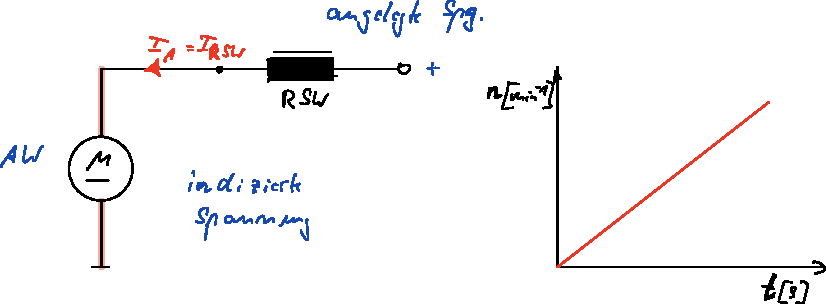
\includegraphics[width=0.6\textwidth]{images/Skizze/30_FT_Reihenschlussmotor.pdf}
\caption{Reihenschlussmotor}
%\label{fig:}%% anpassen
\end{figure}

\subsection{Doppelschlussmotor}\label{doppelschlussmotor}

Hohe Leistung

Kennlinie - Drehzahlverhalten

\begin{figure}[!ht]% hier: !ht
\centering
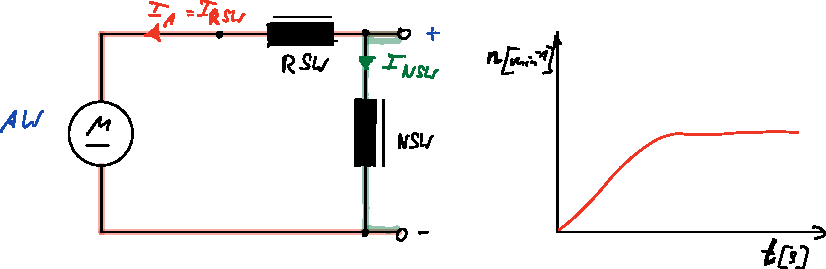
\includegraphics[width=0.6\textwidth]{images/Skizze/30_FT_Doppelschlussmotor.pdf}
\caption{Doppelschlussmotor}
%\label{fig:}%% anpassen
\end{figure}

\subsection{Wechselstrommotor}\label{wechselstrommotor}

Kennlinie - Drehzahlverhalten

\begin{figure}[!ht]% hier: !ht
\centering
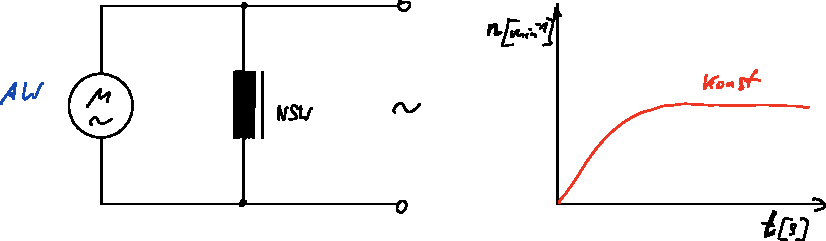
\includegraphics[width=0.6\textwidth]{images/Skizze/30_FT_Wechselstrommotor.pdf}
\caption{Wechselstrommotor}
%\label{fig:}%% anpassen
\end{figure}

\subsection{Schrittmotor}\label{schrittmotor}

Anwendung: Sitzverstellung, Scheinwerferhöhenverstellung, Schiebedach

Kennlinie - Drehzahlverhalten

\begin{figure}[!ht]% hier: !ht
\centering
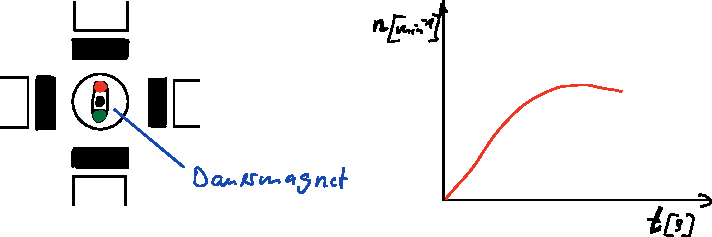
\includegraphics[width=0.6\textwidth]{images/Skizze/30_FT_Schrittmotor.pdf}
\caption{Schrittmotor}
%\label{fig:}%% anpassen
\end{figure}

\subsection{Drehstrommotor}\label{drehstrommotor}

Dozentenwechsel \ldots{}
 \newpage


\chapter{Formelsammlung}
%ju 28-Mai-22 FS-Elektrik.tex
\section{Grundlagen}\label{grundlagen}

\textbf{Eingabe Rechner}

\begin{enumerate}
\def\labelenumi{\alph{enumi}.}
\setcounter{enumi}{25}
\item
  B. $20~mV = \num{20,0e-3} \curvearrowright$ Rechner:
  $20\text{EE}-3 = 0,02$
\end{enumerate}

$10^3 = 1.000 = \num{1,0e3}$

$10^{-3} = \frac{1}{1000} = 0,001 = \num{1,0e-3}$

$10^6 = 1.000.000 = \num{1,0e6}$

$10^{-6} = \frac{1}{1.000.000} = 0,000.001 = \num{1,0e6}$

\textbf{Größen}

$\boxed{K = \num{1,0e3} \quad M = \num{1,0e6} \quad G = \num{1,0e9} \quad T = \num{1,0e12}}$

$\boxed{m = \num{1,0e-3} \quad \mu = \num{1,0e-6} \quad n = \num{1,0e-9} \quad p = \num{1,0e-12}}$

\textbf{Einheiten}

\textbf{Faktor} Länge 10, Fläche 100, Volumen 1000

$\boxed{\mu m \quad mm \quad cm \quad dm \quad m \quad km}$

$1~l = 1~dm^3 \quad 10~ml = 1~cl = 0,01~l$

$\frac{g}{cm^3} \quad \frac{kg}{dm^3} \quad \frac{t}{m^3}$

\textbf{Prozent} $10~\% = \frac{10}{100} = 0,1$

\textbf{km/h in m/s}
$\Rightarrow \frac{km/h}{3,6} \quad \frac{km}{h} \Rightarrow \frac{m}{s} \Rightarrow \frac{1000}{3600}$

\textbf{Stunden:Min:Sek in Dezimalstunden}
$\Rightarrow \text{h} + \frac{Min}{60} + \frac{Sek}{60 \cdot 60}$

\textbf{Zoll in mm} $1~\text{Zoll} = 25,4~mm$

\textbf{Kreisfläche}
$\boxed{\frac{d^2 \cdot \pi}{4}} \quad \text{Hinweis: }\frac{\pi}{4} \approx 0,785$

\textbf{Masse} $\boxed{m = V \cdot \rho}$ Dichte bleibt immer gleich
$\to$ Volumen ändert sich

\textbf{Volumen} $\boxed{V = A \cdot h}$

\textbf{Umfang} $\boxed{Umfang = d \cdot \pi}$

\textbf{Drehmoment} $\boxed{M = F \cdot r}$

\section{Fach Elektrotechnik}\label{fach-elektrotechnik}

\textbf{SPANNUNG} $U~\text{Volt}~[V]$

\textbf{STROM} $I~\text{Ampere}~[A]$

\textbf{WIDERSTAND} $R~\text{Ohm}~[\Omega]$

\textbf{Reihe}

\begin{enumerate}
\item
  Strombegrenzung
\item
  Spannungsteilung
\end{enumerate}

\textbf{Parallel}

\begin{enumerate}
\item
  Stromflusserhöhung
\item
  Leistungsteilung $\boxed{R_{ges} = \frac{R_{Teil}}{n}}$
\end{enumerate}

\textbf{OHMSCHE GESETZ}

$\boxed{I = \frac{U}{R}} \quad \bigl[\frac{V}{\Omega}\bigl] = A \quad  \boxed{R = \frac{U}{I}} \quad \bigl[\frac{V}{A}\bigl] = \Omega \quad  \boxed{U = R \cdot I} \quad [\Omega \cdot A] = V$

\textbf{STROMDICHTE}

$\boxed{J = \frac{I}{A}} \quad \bigl[\frac{A}{mm^2}\bigl] \quad  \boxed{I = J \cdot A} \quad \bigl[\frac{A \cdot mm^2}{mm^2}\bigl] = A \quad  \boxed{A = \frac{I}{J}} \quad \bigl[\frac{A \cdot mm^2}{A}\bigl] = mm^2$

\textbf{LEITWERT} $S$ Siemens

$\boxed{G = \frac{1}{R}} \quad \bigl[\frac{1}{\Omega}\bigl] = S \quad \boxed{R = \frac{1}{G}} \quad \bigl[\frac{1}{S} = \Omega\bigl]$

\textbf{LEITERWIDERSTAND}

$\boxed{R_l = \frac{\rho \cdot l}{A}} \quad \bigl[\frac{\Omega \cdot mm^2 \cdot m}{m \cdot mm^2}\bigl] = \Omega \quad \boxed{A = \frac{\rho \cdot l}{R_l}} \quad \bigl[\frac{\Omega \cdot mm^2 \cdot m}{m \cdot \Omega}\bigl] = mm^2$

$\boxed{l = \frac{R_l \cdot A}{\rho}} \quad \bigl[\frac{\Omega \cdot mm^2 \cdot m}{\Omega \cdot mm^2}\bigl] = m$

\textbf{SPEZIFISCHER WIDERSTAND} $\rho$ rho

$\rho \quad \bigl[\frac{\Omega \cdot mm^2}{m}\bigl] \quad \rho_{Cu} = 0,0178~\frac{\Omega \cdot mm^2}{m}$

\textbf{ELEKTRISCHE LEITFÄHIGKEIT} $\kappa$ Kappa

$\boxed{\kappa = \frac{1}{\rho}} \quad \bigl[\frac{m}{\Omega \cdot mm^2}\bigl] \quad \kappa_{Cu} = 56~\frac{m}{\Omega \cdot mm^2}$

\textbf{REIHENSCHALTUNG}

$\boxed{U_{ges} = U_{R_1} + U_{R_2} + U_{R_3} + \dots + U_{R_n}} \quad \bigl[V + V + V\bigl] = V$

$\boxed{U_{teil} = \frac{U_{ges}}{n}} \quad \bigl[\frac{V}{1}\bigl] = V$

$\boxed{I_{ges} = I_{R_1} = I_{R_2} = I_{R_3} = \dots = I_{R_n}} \quad \bigl[A = A = A\bigl] = A$

$\boxed{R_{ges} = R_1 + R_2 + R_3 + \dots + R_n} \quad \bigl[\Omega + \Omega + \Omega\bigl] = \Omega$

\textbf{SPANNUNGSVERLUST} (Spannungsfall)

$U_{ges} = U_v + U_k;\quad U_k = U_{ges} - U_v;\quad U_v = U_{ges} - U_k$

$U_v = R_l \cdot I;\quad R_l = \frac{\rho \cdot l}{A} \quad \bigl[\frac{\Omega \cdot mm^2 \cdot m}{m \cdot mm^2}\bigl] = \Omega$

$U_k = U_{ges} - R_l \cdot I$

$\boxed{U_v = \frac{\rho \cdot l \cdot I}{A}} \quad \bigl[\frac{\Omega \cdot mm^2 \cdot m \cdot A}{m \cdot mm^2}\bigl] = V \quad \rho_{Cu} = 0,0178~\frac{\Omega \cdot mm^2}{m}$

$U_{v_{~\%}} = \frac{U_v \cdot 100}{U_{ges}} \quad \bigl[\frac{V \cdot ~\%}{V}\bigl] = ~\%$

$\boxed{U_{v_{max}} = 0,5~V}$

$\boxed{\text{max. Leiterwiderstand} = 1~\Omega}$ (außer
Starterhauptleitung)

\textbf{INNENWIDERSTAND} (von Spannungsquellen)

$U_q = U_k + U_i \quad [V + V] = V$

$U_k = U_q - U_i \quad [V - V] = V$

$U_i = U_q - U_k \quad [V - V] = V$

$U_i = I \cdot R_i \quad [A \cdot \Omega] = V$

$U_k = I \cdot R_a \quad [A \cdot \Omega] = V$

$I = \frac{U_i}{R_i} \quad [\frac{V}{\Omega}] = A$

$I = \frac{U_k}{R_a} \quad [\frac{V}{\Omega}] = A$

$I = \frac{U_q}{R_{ges}} \quad [\frac{V}{\Omega}] = A$

$I = \frac{U_q}{R_i + R_a} \quad [\frac{V}{\Omega + \Omega}] = A$

$\boxed{U_k = U_q - I \cdot R_i} \quad [V - A \cdot \Omega \to V - V] = V$

$\boxed{R_i = \frac{U_i}{I}} \quad [\frac{V}{A}] = \Omega$

$\boxed{U_k = U_q - U_i - U_v} \quad \boxed{R_{ges} = R_i + R_l + R_\text{ü} + R_{La}}$

\emph{Herleitung}

$U_k = U_q - I \cdot R_i$ $\quad | +I \cdot R_i$

$U_k + I \cdot R_i = U_q - I \cdot R_i + I \cdot R_i$ $\quad | -U_k$

$-U_k + U_k + I \cdot R_i = U_q - U_k$ $\quad | :I$

$\frac{I \cdot R_i}{I} = \frac{U_q - U_k}{I}$
$\quad \bigl[\frac{V - V}{A} \to \frac{V}{A}\bigl] = \Omega$

$R_i = \frac{U_i}{I}$

\textbf{PARALLELSCHALTUNG}

$\boxed{I_{ges} = I_{R_1} + I_{R_2} + I_{R_3} + \dots + I_{R_n}}\quad [A + A + A] = A$

$\boxed{U_{ges} = U_{R_1} = U_{R_2} = U_{R_3} = \dots = U_{R_n}}\quad [V = V = V] = V$

$\boxed{R_{ges} = \frac{1}{\frac{1}{R_1} + \frac{1}{R_2} + \frac{1}{R_3} + \dots + \frac{1}{R_n}}} \quad \bigl[\frac{1}{\frac{1}{\Omega} + \frac{1}{\Omega} + \frac{1}{\Omega}} = \frac{1}{\frac{1}{\Omega}} = \frac{1}{S}\bigl] = \Omega$

Ersatzwiderstand
$\boxed{R_{ges} = \frac{R_{Teil}}{n}} \quad \bigl[\frac{\Omega}{1}\bigl] = \Omega \quad \to \text{Anzahl } n = \frac{R_{Teil}}{R_{ges}} \quad \bigl[\frac{\Omega}{\Omega}\bigl] = 1$

n = Anzahl der Widerstände (gleich große Widerstände)

$\boxed{R_{ges} = \frac{R_1 \cdot R_2}{R_1 + R_2}}$

$R_{ges} = \frac{1}{\frac{1}{R_1} + \frac{1}{R_2} + \frac{1}{R_3}}$

$\to R_{1} = \frac{1}{\frac{1}{R_{ges}} - \frac{1}{R_2} - \frac{1}{R_3}} \quad \to R_{2} = \frac{1}{\frac{1}{R_{ges}} - \frac{1}{R_1} - \frac{1}{R_3}} \quad \to R_{3} = \frac{1}{\frac{1}{R_{ges}} - \frac{1}{R_1} - \frac{1}{R_2}}$

\textbf{LEISTUNG} $P$ (Power) Watt, $[W], [kW]$

$\boxed{P = U \cdot I} \quad [V \cdot A] = W$

$\boxed{U = \frac{P}{I}} \quad [\frac{W}{A} \to \frac{V \cdot A}{A}] = V$

$\boxed{I = \frac{P}{U}} \quad [\frac{W}{V} \to \frac{V \cdot A}{V}] = A$

\textbf{wenn $I$ fehlt} (Einsetzverfahren)

$P = U \cdot I \quad [V \cdot A] = W, \quad I = \frac{U}{R} \quad [\frac{V}{\Omega}] = A$

$P = U \cdot \frac{U}{R} \to \boxed{P = \frac{U^2}{R}} \quad [\frac{V \cdot V}{\Omega} \to A \cdot V] = W$

\textbf{wenn $U$ fehlt} (Einsetzverfahren)

$P = U \cdot I \quad [V \cdot A] = W, \quad U = R \cdot I \quad [\Omega \cdot A] = V$

$P = R \cdot I \cdot I \to \boxed{P = R \cdot I^2} \quad [\Omega \cdot A \cdot A \to V \cdot A] = W$

\textbf{Lampe} $12~V/55~W$

\begin{enumerate}
\item
  $R_{La} = \frac{U^2}{P}$
\item
  $I_{tat} = \frac{U_k}{R_{La}} = \frac{U_{ges} - U_v}{R_{La}}$
\item
  $P_{tat} = U_k \cdot I_{tat}$
\end{enumerate}
 \newpage


\chapter{FM - Übungen}
%ju 28-Mai-22 FM_U01_OhmschesGesetz_Loesung.tex
\section{Ohmsche Gesetz Übung 1}\label{ohmsche-gesetz-uebung-1}

\textbf{Aufgabe 1}

geg:

$R = 45~\Omega, I = 0,32555~A$

ges: $U \text{ in } V$

Lösung:

$U = R \cdot I = 14,6498 V$

\textbf{Aufgabe 2}

geg:

$U = 14,25~V, I = 54,37~A$

ges: $R \text{ in } \Omega$

Lösung:

$R = \frac{U}{I} = 0,2621~\Omega$

\textbf{Aufgabe 3}

geg:

$U = 260~V = 0,26~kV$

$R = 5000~\Omega = 5~k\Omega$

ges: $I \text{ in } A$

Lösung:

$I = \frac{U}{R} = 0,052~A$

\newpage

\textbf{Aufgabe 4}

geg:

$R = 470~\Omega, I = 0,03021~A = 30,21~mA$

ges: $U \text{ in } V$

Lösung:

$U = R \cdot I = 14,1987~V$

\textbf{Aufgabe 5}

geg:

$U_1 = 14,82~V$ \verb|// 100 \%|

$U_2 = \text{?}$
\verb|// 60 \% = 0,6 (-40 \% Abnahme)|

$R = 6,85~\Omega$

ges: $U_2, I_1, I_2, I_{delta}$

Lösung:

$U_2 = U_1 \cdot 0,6 = 8,892~V$

$I_1 = \frac{U_1}{R} = 2,1635~A$

$I_2 = \frac{U_2}{R} = 1,2981~A$

$I_{delta} = I_1 - I_2 = 0,8654~A$

\textbf{Aufgabe 6}

geg:

$U = 14,2~V$

$R_{E_{12}} = 2,618~\Omega, R_{K_2} = 72~\Omega$

ges: $I_{Steuer}, I_{F_2}$

Lösung:

$I_{Steuer} = \frac{U}{R_{K_2}} = 0,1972~A$

$I_{F_2} = \frac{U}{R_{E_{12}}} = 5,424~A$

\newpage

\textbf{Aufgabe 7}

geg:

$I_{delta} = 4,32~A$

$R_{kalt} = 0,86~\Omega$

$U = 13,8~V$

ges: $I_{kalt},\, I_{warm}, R_{warm}, R_{delta}$

Lösung:

$I_{kalt} = \frac{U}{R_{kalt}} = 16,0465~A$

$I_{warm} = I_{kalt} - I_{delta} = 11,7265~A$

$R_{warm} = \frac{U}{I_{warm}} = 1,1768~\Omega$

$R_{delta} = R_{warm} - R_{kalt} = 0,3168~\Omega$
 \newpage
%ju 28-Mai-22 FM_U02_Leiterwiderstand_Loesung.tex
\section{Leiterwiderstand Übung 2}\label{leiterwiderstand-uebung-2}

\textbf{Aufgabe 1}

geg:

$l = 8,25~m$

$A = 0,75~mm^2$

$\rho = 0,0178~\frac{\Omega \cdot mm^2}{m} \,\text{(Kupfer)}$

ges: $R_l$

Formel

$R_l = \frac{p \cdot l}{A}$

Lösung

$R_l = 0,1958~\Omega$

\textbf{Aufgabe 2}

geg:

$R_l = 0,3648~m\Omega = 0,0003648~\Omega = \num{3,648e-04}~\Omega$

$\rho = 0,0178~\frac{\Omega \cdot mm^2}{m} \,\text{(Kupfer)}$

$d = 12,363~mm$

ges: $A, l$

Formel

$A = d^2 \cdot \pi$ oder $A = d^2 \cdot 0,785 \to (pi/4 = 0,785)$

$R_l = \frac{p \cdot l}{A} \to l = \frac{R_l \cdot A}{p}$

Lösung

$l = 2,459~m$

\textbf{Aufgabe 3}

geg:

$l = 4,5~m$

$R_l = 0,00267~\Omega = 2,666666~m\Omega = \num{2,67e-03}~\Omega$

$\rho = 0,0178~\frac{\Omega \cdot mm^2}{m} \,\text{(Kupfer)}$

ges: $A$

Formel

$R_l = \frac{p \cdot l}{A} \to A = \frac{p \cdot l}{R_l}$

Lösung

$A = 30,0~mm^2$

\textbf{Aufgabe 4}

\begin{figure}[!ht]% hier: !ht
\centering
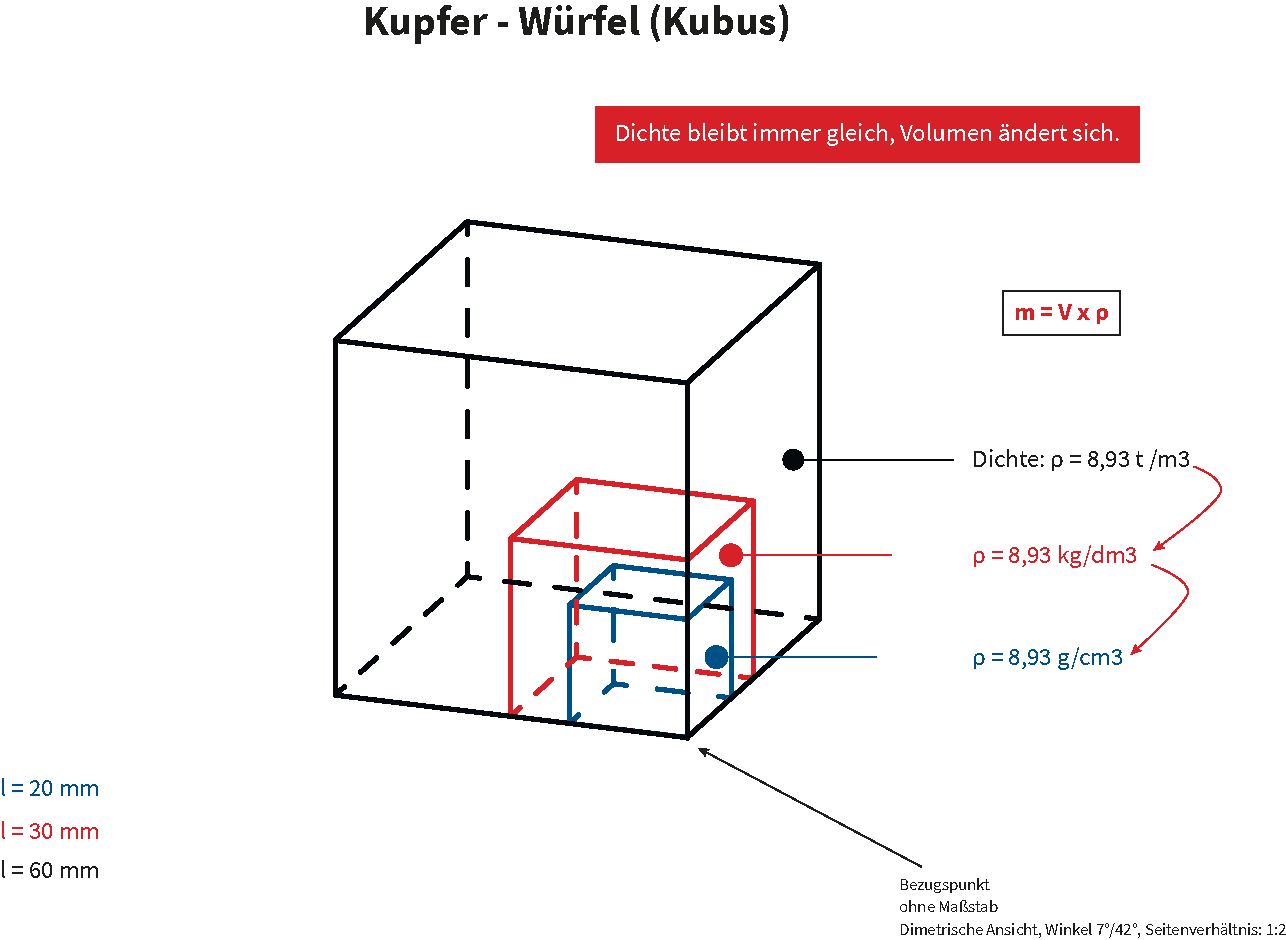
\includegraphics[width=0.6\textwidth]{images/Skizze/Kupfer_Wuerfel_Dichte.pdf}
\caption{Dichte / Volumen eines Kupferwürfels}
%\label{fig:}%% anpassen
\end{figure}

$\boxed{l = 2~cm}, V = (2~cm)^3 = 8~cm^3$

$m = 8~cm^3 \cdot 8,93~\frac{g}{cm^3} = 71~g$

$\boxed{l = 3~cm} = 0,3~dm, V = (0,3~dm)^3 = 0,027~dm^3$

$m = 0,027~dm^3 \cdot 8,93~\frac{kg}{dm^3} = 0,241~kg = 241~g$

$\boxed{l = 6~cm} = 0,06~m, V = (0,06~m)^3 = 0,000216~m^3$

$m = 0,000216~m^3 \cdot 8,93~\frac{t}{m^3} = 0,001929~t = 1929~g$

geg: Spule

$d_m = 36~mm = 3,6~cm$

$N = 1480$ (Windungen)

$d_D = 0,36~mm$

$p_{cu} = 8,93~\frac{t}{m^3}$ (Dichte)

$\rho = 0,0178~\frac{\Omega \cdot mm^2}{m} \,\text{(Kupfer)}$

ges: $A, l, R_l, G, V, m$

Formel

\emph{Kreisringfläche}: D = Außendurchmesser; d = Innendurchmesser; r =
Radius; $d_{mitte} = d_m$

$U = d \cdot \pi; \quad d_m = \frac{(D+d)}{2}; \quad r_m = \frac{(D+d)}{4}$

$A = \frac{d_D^2 \cdot \pi}{4}$

$l = U \cdot N \to l = \frac{d_m}{10} \cdot \pi \cdot N$

$R_l = \frac{\rho \cdot l}{100 \cdot A}$

$G = \frac{1}{R_l}$

$V = A \cdot h \to V = \frac{A}{100} \cdot l$

$m = V \cdot p_{cu}$

Lösung

$A = 0,1018~mm^2$

$l = 16738,4057~cm$

$R_l = 29,2711~\Omega$

$G = 0,0342~S$

$V = 17,0376~cm^3$

$m = 152,146~g$

\textbf{Aufgabe 5,1}

geg:

$R_l = 13,171999~m\Omega = 0,013171999~\Omega = \num{1,3171999e-2}~\Omega$

$\rho = 0,0178~\frac{\Omega \cdot mm^2}{m} \,\text{(Kupfer)}$

$d = 1,784576526~mm$

ges: $A, l$

Formel

$A = d^2 \cdot 0,785 \to (pi/4 = 0,785)$

$R_l = \frac{\rho \cdot l}{A} \to l = \frac{R_l \cdot A}{\rho}$

Lösung

$l = 1,85~m$

\textbf{Aufgabe 5,2}

Gleiche Leiterfläche für die Rückleitung, dass sie genauso hoch belastet
wird wie die positive Versorgungsleitung,

Sie liegen beide in Reihe, werden also vom gleichen Strom durchflossen,
 \newpage
%ju 28-Mai-22 FM_U03_Reihenschaltung_Loesung.tex
\section{Reihenschaltung Übung 3}\label{reihenschaltung-uebung-3}

\textbf{Aufgabe 1}

geg:

$R_1 = 40~\Omega, R_2 = 110~\Omega, R_3 = 50~\Omega$

$U_2 = 4,4~V$

ges: $I, U_1, U_3$

Formel

$I = \frac{U_2}{R_2}$

$U_1 = R_1 \cdot I, U_3 = R_3 \cdot I$

Lösung:

$I = 0,04~A$

$U_1 = 1,6~V, U_3 = 2,0~V$

\textbf{Aufgabe 2}

geg:

$R_1 = 8~\Omega, R_2 = 24~\Omega$

$U_{ges} = 12~V$

$I = 0,27~A = 270~mA$

ges: $R_{ges}, R_3, U_1, U_2, U_3$

Formel

$R_{ges} = \frac{U_{ges}}{I}$

$R_{ges} = R_1 + R_2 + R_3 \to R_3 = R_{ges} - R_1 - R_2$

$U_1 = R_1 \cdot I, U_2 = R_2 \cdot I, U_3 = R_3 \cdot I$

Lösung:

$R_{ges} = 44,4444~\Omega, R_3 = 12,4444~\Omega$

$U_1 = 2,16~V, U_2 = 6,48~V, U_3 = 3,36~V$

\newpage

\textbf{Aufgabe 3}

\begin{figure}[!ht]% hier: !ht
\centering
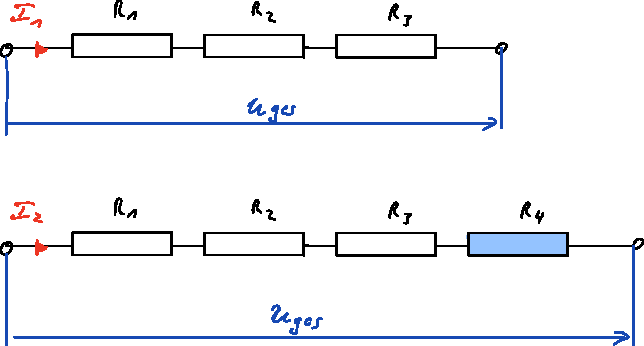
\includegraphics[width=0.6\textwidth]{images/Skizze/22_FM_Nr3_Reihenschaltung_Aufg3_Skizze.pdf}
\caption{Schaltung Reihenschaltung Aufgabe 3}
%\label{fig:}%% anpassen
\end{figure}

geg:

$R_1 = R_2 = R_3 = 22~\Omega$

$I_1 = 0,87~A = 870~mA$

$I_{delta} = 0,075~A = 75~mA$

ges: $I_2, R_{ges_1}, U_{ges}, R_{ges_2}, R_4, U_1, U_2, U_3, U_4$

Formel

$I_2 = I_1 - I_{delta}$

$R_{ges_1} = R_1 + R_2 + R_3$

$U_{ges} = R_{ges_1} \cdot I_1$

$R_{ges_2} = \frac{U_{ges}}{I_2}$

$R_{ges_2} = R_1 + R_2 + R_3 + R_4 \to R_4 = R_{ges_2} - R_1 - R_2 - R_3$

$U_4 = R_4 \cdot I_2$

$U_1 = R_1 \cdot I_2$

Lösung:

$I_2 = 0,795~A$

$R_{ges1} = 66~\Omega$

$U_{ges} = 57,42~V$

$R_{ges2} = 72,2264~\Omega$

$R_4 = 6,2264~\Omega$

$U_4 = 4,95~V$

$U_1 = 17,49~V \to R_1 = R_2 = R_3 \to U_1 = U_2 = U_3$

\newpage

\textbf{Aufgabe 4}

\begin{figure}[!ht]% hier: !ht
\centering
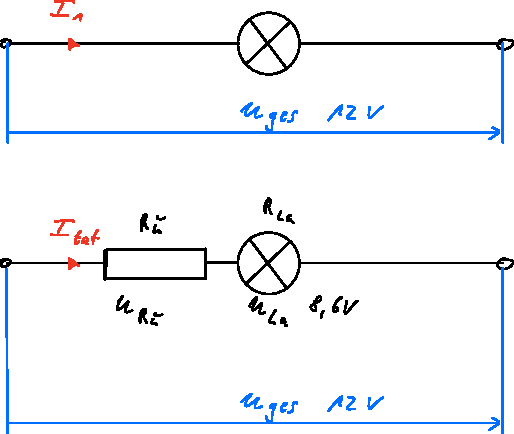
\includegraphics[width=0.6\textwidth]{images/Skizze/23_FM_Nr3_Reihenschaltung_Aufg4_Skizze.pdf}
\caption{Schaltung Reihenschaltung Aufgabe 4}
%\label{fig:}%% anpassen
\end{figure}

geg:

$U_{ges} = 12~V$

$I_1 = 1,75~A$

$U_{La} = 8,6~V$

ges: $U_{R_\text{ü}}, R_{La}, I_{tat}, R_\text{ü}$

Formel

$U_{ges} = U_{La} + U_{R_\text{ü}} \to U_{R_\text{ü}} = U_{ges} - U_{La}$

$R_{La} = \frac{U_{ges}}{I_1}$

$I_{tat} = \frac{U_{La}}{R_{La}}$

$R_\text{ü} = \frac{U_{R_\text{ü}}}{I_{tat}}$

Lösung:

$U_{R_\text{ü}} = 3,4~V$

$R_{La} = 6,8571~\Omega$

$I_{tat} = 1,2542~A$

$R_\text{ü} = 2,711~\Omega$
 \newpage
%ju 28-Mai-22 FM_U03_Reihenschaltung_Mathebuch_Loesung.tex
\section{Reihenschaltung Übung 3
Mathebuch}\label{reihenschaltung-uebung-3-mathebuch}

Vgl. Mathebuch (\textcite{elbl:2016:technMa} S.82)

\textbf{Aufgabe 1}

geg:

$R_1 = 125~\Omega, R_2 = 250~\Omega$

$U = 225~V$

ges: $R_{ges}, I, U_1, U_2$

Formel

$R_{ges} = R_1 + R_2$

$I = \frac{U}{R_{ges}}$

$U_1 = R_1 \cdot I, U_2 = R_2 \cdot I$

Lösung:

$R_{ges} = 375~\Omega$

$I = 0,6~A$

$U_1 = 75,0~V, U_2 = 150,0~V$

\textbf{Aufgabe 2}

geg:

$U_{ges} = 235~V$

$R_1 = 176~\Omega$

$I = 0,25~A$

ges: $U_1, U_2, R_2$

Formel

$U_1 = R_1 \cdot I$

$U_{ges} = U_1 + U_2 \to U_2 = U_{ges} - U_1$

$R_2 = \frac{U_2}{I}$

Lösung:

$U_1 = 44,0~V, U_2 = 191,0~V$

$R_2 = 764,0~\Omega$
 \newpage
%ju 28-Mai-22 FM_U04_Spannungsabfall_Loesung.tex
\section{Spannungsabfall Übung 4}\label{spannungsabfall-uebung-4}

Tabellenbuch S. 280 Nennquerschnitt

\textbf{Aufgabe 1}

geg:

$A = 0,6~mm^2$

$\rho = 0,3~\frac{\Omega \cdot mm^2}{m}$

$I = 8~A$

$U_v = 4~V$

ges: $l$

Formel:

$U_v = \frac{\rho \cdot l \cdot I}{A} \to l = \frac{U_v \cdot A}{\rho \cdot I}$

Lösung:

$l = 1,0~m$

\textbf{Aufgabe 2}

geg:

$l = 4~m$ (Kupfer)

$U_{ges} = 10~V, U_k = 9,6~V$

$I = 150~A$

$\rho = 0,0178~\frac{\Omega \cdot mm^2}{m}$

ges: $R_{st}, A_{mind}, A_{Nenn}$

Formel:

$R_{st} = \frac{U_k}{I}$

$U_v = U_{ges} - U_k \to A_{mind} = \frac{\rho \cdot l \cdot I}{U_v} \to A_{mind} = \frac{\rho \cdot l \cdot I}{(U_{ges} - U_k)}$

Lösung:

$R_{st} = 0,064~\Omega$

$A_{mind} = 26,7~mm^2 \to A_{Nenn} = 35~mm^2$ (Nennquerschnitt)

\newpage

\textbf{Aufgabe 3}

geg:

$A = 0,75~mm^2$

$l = 6~m$ (Kupfer)

$U_v = 0,3~V = 300 mV$

$\rho = 0,0178~\frac{\Omega \cdot mm^2}{m}$

ges: $I$

Formel:

$U_v = \frac{\rho \cdot l \cdot I}{A} \to I = \frac{U_v \cdot A}{\rho \cdot l}$

Lösung:

$I = 2,1067~A$

\textbf{Aufgabe 4}

\begin{figure}[!ht]% hier: !ht
\centering
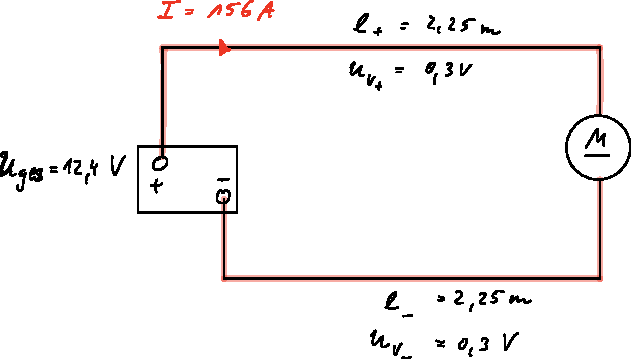
\includegraphics[width=0.6\textwidth]{images/Skizze/24_FM_Nr4_Reihenschaltung_Aufg4_Skizze.pdf}
\caption{Schaltung Spannungsabfall Aufgabe 4}
%\label{fig:}%% anpassen
\end{figure}

geg:

$l = 4,5~m$ (Kupfer), $l_1 = 2,25~m$ (Plusleitung), $l_2 = 2,25~m$
(Minusleitung)

$U_v = 0,3~V, U_B = 12,4~V$

$\rho = 0,0178~\frac{\Omega \cdot mm^2}{m}$

$I = 156~A$

ges: $R_{st}, A_{mind}, A_{Nenn}$

Formel:

$U_k = U_B - U_{v_+} - U_{v_-} \to R_{st} = \frac{U_k}{I} \to R_{st} = \frac{(U_B - U_{v_+} - U_{v_-})}{I}$

$U_v = \frac{\rho \cdot l \cdot I}{A} \to A_{mind} = \frac{\rho \cdot l_1 \cdot I}{U_v}$

Lösung:

$R_{st} = 0,0756~\Omega$

$A_{mind} = 20,826~mm^2 \to A_{Nenn} = 25~mm^2$ (Nennquerschnitt)

\newpage

\textbf{Aufgabe 5}

geg:

$l = 1,65~m$ (Kupfer)

$U_{v_\%} = 2,5~\% \text{ von } 12~V$

$U_{ges} = 12~V$

$\rho = 0,0178~\frac{\Omega \cdot mm^2}{m}$

$I = 50~A$

ges: $U_v, A_{mind}, A_{Nenn}$

Formel:

$U_{v_\%} = \frac{U_v \cdot 100}{U_{ges}} \to U_v = \frac{U_{v_\%} \cdot U_{ges}}{100}$

$U_v = \frac{\rho \cdot l \cdot I}{A} \to A_{mind} = \frac{\rho \cdot l \cdot I}{U_v}$

Lösung:

$U_v = 0,3~V$

$A_{mind} = 4,895~mm^2 \to A_{Nenn} = 6~mm^2$ (Nennquerschnitt)

\textbf{Aufgabe 6}

geg:

$U_v = 0,10385232~V = 103,85232~mV$

$\rho = 0,0178~\frac{\Omega \cdot mm^2}{m}$

$I = 1,87~A$

$A = 1,5~mm^2$

ges: $l$

Formel:

$U_v = \frac{\rho \cdot l \cdot I}{A} \to l = \frac{U_v \cdot A}{\rho \cdot I}$

Lösung:

$l = 4,68~m$
 \newpage
%ju 28-Mai-22 FM_U04_Spannungsabfall_Mathebuch_Loesung.tex
\section{Spannungsabfall Übung 4
Mathebuch}\label{spannungsabfall-uebung-4-mathebuch}

Vgl. Mathebuch (\textcite{elbl:2016:technMa} S. 107)

\textbf{Aufgabe 1}

Schaltung Spannungsverlust

\begin{figure}[!ht]% hier: !ht
\centering
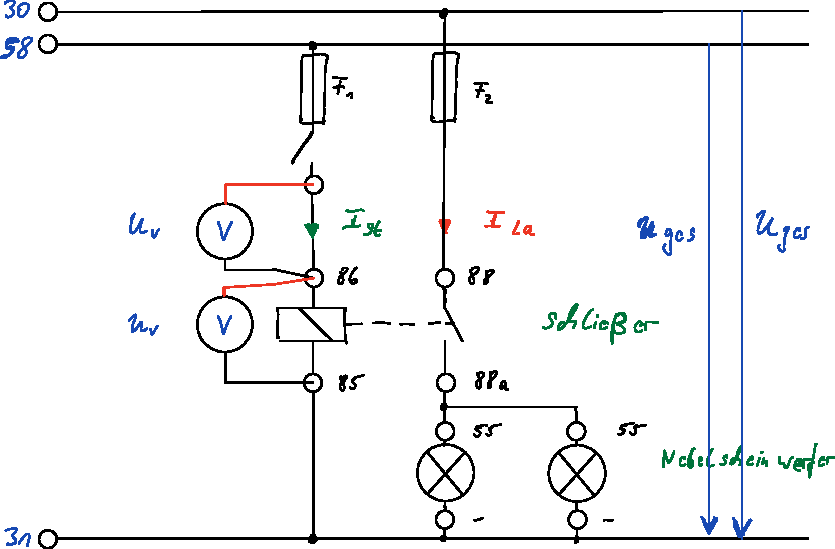
\includegraphics[width=0.65\textwidth]{images/Skizze/13_Spannungsverlust_Skizze.pdf}
\caption{Schaltung Spannungsverlust Aufgabe 1}
%\label{fig:}%% anpassen
\end{figure}

Nennquerschnitt Tabellenbuch (\textcite{bell:2021:tabellenbuchKfz} S. 280)

Spannungsfall Tabellenbuch (\textcite{bell:2021:tabellenbuchKfz} S. 280)

geg:

$l_1 = 0,8~m, l_2 = 1,6~m, l_{2}' = 1,6~m$

$U_{v_{l_1}} = 0,1 V, U_{v_{l_2}} = 0,1 V, U_{v_{l_2}}' = 0,1 V$

$P_{La_{22/23}}= 12~V/55~W, P = 55~W, U = 12~V$

$\rho = 0,0178~\frac{\Omega \cdot mm^2}{m} \,\text{(Kupfer)}$

ges:
$I, A_{l_1}, A_{Nenn}, J_{l_1}, A_{l_2}, J_{A_{l_2}}, J_{A_{l_2}}'$

Formel:

$P = U \cdot I \to I = \frac{P}{U}$

$U_{v_{l_1}} = \frac{\rho \cdot l_1 \cdot I}{A_{l_1}} \to A_{l_1} = \frac{\rho \cdot l_1 \cdot 2 \cdot I}{U_{v_{l_1}}}$

$J_{A_{l_2}} = \frac{I}{A_{Nenn}}$

$U_{v_{l_2}} = U_{v_{l_2}}' \to U_{v_{l_2}} = \frac{\rho \cdot l_2 \cdot I}{A_{l_2}} \to A_{l_2} = \frac{\rho \cdot l_2 \cdot I}{U_{v_{l_2}}}$

$J_{A_{l_2}} = J_{A_{l_2}}' \to J_{A_{l_2}} = \frac{I}{A_{Nenn}}$

Lösung:

$I = 4,5833~A$

$A_{l_1} = 1,3053~mm^2 \to A_{Nenn} = 1,5~mm^2$

$J_{l_1} = 6,1111~\frac{A}{mm^2}$

$A_{l_2} = 1,3053~mm^2 \to A_{Nenn} = 1,5~mm^2$

$J_{A_{l_2}} = J_{A_{l_2}}' = 3,0556~\frac{A}{mm^2}$

\textbf{Aufgabe 2}

geg:

$I = 165~A$

$l_{ges} = 1,7 + 3,4~m$ (zwei Kabel)

$U_{v_{max}} = 0,5~V$

$U_{k_{Bat}} = 11,2~V$

$\rho = 0,0178~\frac{\Omega \cdot mm^2}{m} \,\text{(Kupfer)}$

ges: $A_{mind}, A_{Nenn}, U_{v_{mind}}, U_{K_{st}}$

Formel:

$U_v = \frac{\rho \cdot l \cdot I}{A} \to A_{mind} = \frac{\rho \cdot l_{ges} \cdot I}{U_{v_{max}}}$

$U_{v_{mind}} = \frac{\rho \cdot l_{ges} \cdot I}{A_{mind}} \quad \text{vs.} \quad U_{v_{Nenn}} = \frac{\rho \cdot l_{ges} \cdot I}{A_{Nenn}}$

$U_{K_{st}} = U_{k_{Bat}} - U_{v_{Nenn}}$

Lösung:

$A = 29,9574~mm^2 \to A_{Nenn} = 35~mm^2$ (Nennquerschnitt)

$U_{v_{mind}} = 0,5~V \quad \text{vs.} \quad U_{v_{Nenn}} = 0,428~V$

$U_{K_{st}} = 10,772~V$
 \newpage
%ju 28-Mai-22 FM_U05_Innenwiderstand_Loesung.tex
\section{Innenwiderstand Übung 5}\label{innenwiderstand-uebung-5}

\textbf{Aufgabe 1}

Ein $24~V$ Starter wird über zwei $12~V$ Batterien mit elektrischer
Energie versorgt. Die Batteriezellen besitzen einen Innenwiderstand von
$0,74~m\Omega$/Zelle. Durch die $2,3~m$ lange Versorgungsleitung mit
einer Fläche von $120~mm^2$ fließt ein Strom von $1250~A$.

Wie groß ist die Klemmenspannung am Starter?

\begin{figure}[!ht]% hier: !ht
\centering
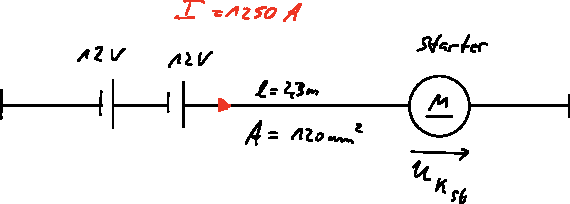
\includegraphics[width=0.6\textwidth]{images/Skizze/20_FM_Nr5_Innenwiderstand_Aufg1_Skizze.pdf}
\caption{Schaltung Innenwiderstand Aufgabe 1}
%\label{fig:}%% anpassen
\end{figure}

geg:

$R_{i_{zelle}} = 0,00074~\Omega = 0,74~m \Omega /Zelle$

$U_{{Bat}_1} = 12~V$

$U_{{Bat}_2}= 12~V$

$z = 12$ (Anzahl Batteriezellen)

$I = 1250~A$

$l = 2,3~m$

$A = 120~mm^2$

$\rho = 0,0178~\frac{\Omega \cdot mm^2}{m}$

ges: $U_{K_{st}}$

Formel:

$U_i = R_{i_{ges}} \cdot I \quad \to U_i = R_{i_{zelle}} \cdot z \cdot I$

$U_v = \frac{I \cdot \rho \cdot l}{A}$

$U_{ges} = U_i + U_v + U_{K_{st}} \quad \to U_{K_{st}} = U_{{Bat}_1} + U_{{Bat}_2} - U_v - U_i$

Lösung:

$U_i = 11,1~V$

$U_v = 0,4265~V$

$U_{K_{st}} = 12,4735~V$

\textbf{Aufgabe 2}

\begin{figure}[!ht]% hier: !ht
\centering
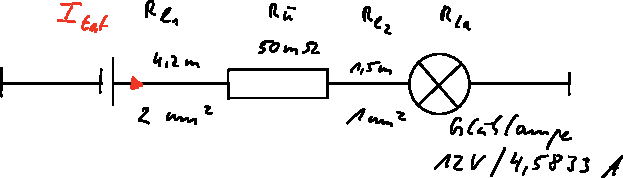
\includegraphics[width=0.6\textwidth]{images/Skizze/21_FM_Nr5_Innenwiderstand_Aufg2_Skizze.pdf}
\caption{Schaltung Innenwiderstand Aufgabe 2}
%\label{fig:}%% anpassen
\end{figure}

geg: Glühlampenaufschrift: $12~V / 4,5833~A$

$U = 12~V$

$I = 4,5833~A$

$U_q = 14,8~V$

$R_i = 0,012~\Omega = 12~m \Omega$

$A_1 = 2~mm^2, A_2 = 1~mm^2$

$l_1 = 4,2~m, l_2 = 1,5~m$

$R_\text{ü} = 0,050~\Omega = 50~m \Omega$

$\rho = 0,0178~\frac{\Omega \cdot mm^2}{m}$

ges: Mit welcher Klemmenspannung wird die Schaltung gespeist?

Formel:

$R_{l_1} = \frac{\rho \cdot l_1}{A_1}, R_{l_2} = \frac{\rho \cdot l_2}{A_2}$

$R_{La} = \frac{U}{I}$

$R_{ges} = R_i + R_{l_1} + R_\text{ü} + R_{l_2} + R_{La}$

$I_{tat} = \frac{U_q}{R_{ges}}$

$U_K = U_q - I \cdot R_i$

Lösung:

$R_{l_1} = 0,0374~\Omega, R_{l_2} = 0,0267~\Omega$

$R_{La} = 2,6182~\Omega$

$R_{ges} = 2,7443~\Omega$

$I_{tat} = 5,393~A$

$U_K = 14,745~V$
 \newpage
%ju 28-Mai-22 FM_U05_Innenwiderstand_Mathebuch_Loesung.tex
\section{Innenwiderstand Übung 5
Mathebuch}\label{innenwiderstand-uebung-5-mathebuch}

Vgl. Mathebuch (\textcite{elbl:2016:technMa} S. 121)

\textbf{Aufgabe 1}

geg:

$U_q = 12,6~V$

$R_i = 0,012~\Omega = 12~m\Omega$

$R_a = 0,051~\Omega$ (Außenwiderstand)

ges: $I, U_k$

Formel:

$I = \frac{U_q}{R_{ges}} \to I = \frac{U_q}{(R_i + R_a)}$

$U_k = I \cdot R_a$

Lösung:

$I = 200,0 A$

$U_k = 10,2 V$

\textbf{Aufgabe 2}

geg:

$I = 400~A$

$U_q = 12,5~V$

$U_{k_1} = 8,3~V$ (nach 30 s), $U_{k_2} = 6,2~V$ (nach 150 s)

ges: $R_{i_1}, R_{i_2}$

Formel:

$R_{i_1} = \frac{U_{i_1}}{I} \to R_{i_1} = \frac{(U_q - U_{k_1})}{I}$

$R_{i_2} = \frac{U_{i_2}}{I} \to R_{i_2} = \frac{(U_q - U_{k_2})}{I}$

Lösung:

$R_{i_1} = 0,0105~\Omega, R_{i_2} = 0,0158~\Omega$
 \newpage
%ju 28-Mai-22 FM_U06_Parallelschaltung_Loesung.tex
\section{Parallelschaltung Übung 6}\label{parallelschaltung-uebung-6}

\textbf{Aufgabe 1}

geg:

$R_1 = 72~\Omega, R_2 = 48~\Omega$ $R_{ges} = 12~\Omega$

ges: $R_3$

Formel:

$R_{ges} = \frac{1}{(\frac{1}{R_1} + \frac{1}{R_2} + \frac{1}{R_3})} \quad \to R_3 = \frac{1}{(\frac{1}{R_{ges}} - \frac{1}{R_1} - \frac{1}{R_2})}$

Lösung:

$R_3 = 20,5714~\Omega$

\textbf{Aufgabe 2}

geg: \textbar\textbar{}

$R_1 = 30~\Omega, R_2 = 45~\Omega$

$I_1 = 0,45~A$

$I_{ges} = 0,8~A$

ges: $U, R_3, R_{ges}$

Formel:

$U = R_1 \cdot I_1$

$R_{ges} = \frac{U}{I_{ges}}$

$I_2 = \frac{U}{R_2}$

$I_{ges} = I_1 + I_2 + I_3 \quad \to I_3 = I_{ges} - I_1 - I_2$

$R_3 = \frac{U}{I_3}$

Lösung:

$U = 13,5~V$

$R_{ges} = 16,875~\Omega$

$I_2 = 0,3~A, I_3 = 0,05~A$

$R_3 = 270,0~\Omega$

\newpage

\textbf{Aufgabe 3}

geg:

$R_{Teil} = 66~\Omega$

$R_{ges} = 16,5~\Omega$

ges: $n$ (Anzahl)

Formel:

$R_{ges} = \frac{R_{Teil}}{n} \quad \to n = \frac{R_{Teil}}{R_{ges}}$

Lösung:

$n = 4$

\textbf{Aufgabe 4}

geg: \textbar\textbar{}

$R_2 = 3,4515~\Omega$

$I_1 = 0,85~A, I_2 = 4,23~A, I_3 = 1,85~A, I_4 = 2,69~A$

ges: $R_{ges}, R_1, R_4, R_3$

Formel:

$U = R_2 \cdot I_2$

$R_1 = \frac{U}{I_1}, R_3 = \frac{U}{I_3}, R_4 = \frac{U}{I_4}$

$I_{ges} = I_1 + I_2 + I_3 + I_4$

Variante 1: $R_{ges} = \frac{U}{I_{ges}}$ Variante 2:
$R_{ges} = \frac{1}{(\frac{1}{R_1} + \frac{1}{R_2} + \frac{1}{R_3} + \frac{1}{R_4})}$

Lösung:

$U = 14,5998~V$

$R_1 = 17,1763~\Omega, R_3 = 7,8918~\Omega, R_4 = 5,4275~\Omega$

$I_{ges} = 9,62 A$

Variante 1: $R_{ges} = 1,5177~\Omega$ Variante 2:
$R_{ges} = 1,5177~\Omega$

\newpage

\textbf{Aufgabe 5}

geg: \textbar\textbar{} Glühkerze PTC Regelwiderstand $\theta$, x =
Temperatur $\uparrow$, y = Widerstand $\uparrow$

$z = 4$ (Zylinderzahl)

$R_{R_k} = 0,38~\Omega$ (Regelwiderstand kalt)

$R_{R_w} = 0,88~\Omega$ (Regelwiderstand warm)

$R_H = 0,55~\Omega$ \{Heizwendel\}

$U_K = 13,8~V$

ges: $I_{{ges}_k}, I_{{ges}_w}, P_{K_k}, P_{K_w}$

Formel:

$I_{K_k} = \frac{U_K}{R_{K_k}} \quad \to I_{K_k} = \frac{U_K}{(R_{R_k} + R_H)}$

$I_{{ges}_k} = I_{K_k} \cdot z$

$I_{K_k} = \frac{U_K}{R_{K_w}} \quad \to I_{K_w} = \frac{U_K}{(R_{R_w} + R_H)}$

$I_{{ges}_w} = I_{K_w} \cdot z$

$P_{K_k} = U_K \cdot I_{K_k}, P_{K_w} = U_K \cdot I_{K_w}$

Lösung:

$I_{K_k} = 14,8387~A, I_{{ges}_k} = 59,3548~A$

$I_{K_w} = 9,6503~A, I_{{ges}_w} = 38,6014~A$

$P_{K_k} = 204,7742~W$ (Leistung - Glühkerze kalt)
$P_{K_w} = 133,1748~W$ (Leistung - Glühkerze warm)
 \newpage
%ju 28-Mai-22 FM_U06_Parallelschaltung_Mathebuch_Loesung.tex
\section{Parallelschaltung Übung 6
Mathebuch}\label{parallelschaltung-uebung-6-mathebuch}

Vgl. Mathebuch (\textcite{elbl:2016:technMa} S. 82)

\textbf{Aufgabe 4a)}

geg:

$R_1 = 30~\Omega, R_2 = 20~\Omega$

$U = 12,6~V$

ges: $I_{ges}, I_1, I_2, R_{ges}$

Formel:

$I_1 = \frac{U}{R_1}, I_2 = \frac{U}{R_2}$

$I_{ges} = I_1 + I_2$

$R_{ges} = \frac{U}{I_{ges}}$

Lösung:

$I_1 = 0,42~A, I_2 = 0,63~A$

$I_{ges} = 1,05~A$

$R_{ges} = 12,0~\Omega$

\textbf{Aufgabe 4b)}

geg:

$I_1 = 0,3~A, I_2 = 0,2~A$

$U = 14,4~V$

ges: $I_{ges}, R_{ges}, R_1, R_2$

Formel:

$I_{ges} = I_1 + I_2$

$R_{ges} = \frac{U}{I_{ges}}$

$R_1 = \frac{U}{I_1}, R_2 = \frac{U}{I_2}$

Lösung:

$I_{ges} = 0,5~A$

$R_{ges} = 28,8~\Omega$

$R_1 = 48,0~\Omega, R_2 = 72,0~\Omega$

\newpage

\textbf{Aufgabe 4c)}

geg:

$I_{ges} = 1,2~A$

$I_2 = 0,3~A$

$R_{ges} = 187,5~\Omega$

ges: $I_1, R_1, R_2, U$

Formel:

$I_{ges} = I_1 + I_2 \quad \to I_1 = I_{ges} - I_2$

$U = R_{ges} \cdot I_{ges}$

$R_1 = \frac{U}{I_1}, R_2 = \frac{U}{I_2}$

Lösung:

$I_1 = 0,9~A$

$U = 225,0~V$

$R_1 = 250,0~\Omega, R_2 = 750,0~\Omega$
 \newpage
%ju 28-Mai-22 FM_U07_gemischte_Schaltung_Loesung.tex
\section{gemischte Schaltung Übung
7}\label{gemischte-schaltung-uebung-7}

\textbf{Aufgabe 1}

\begin{figure}[!ht]% hier: !ht
\centering
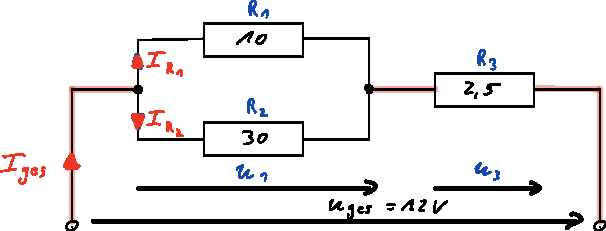
\includegraphics[width=0.6\textwidth]{images/Skizze/25_FM_Nr7_gemischte_Schaltung_A1.pdf}
\caption{FM Nr7 gemischte Schaltung A1}
%\label{fig:}%% anpassen
\end{figure}

\lstset{language=Python}% C, TeX, Bash, Python 
\begin{lstlisting}[
	%caption={}, label={code:}%% anpassen
][language=Python]
# geg: Mathebuch S. 82 Aufgabe 6 Schaltung
R_1 = 10 Ohm
R_2 = 30 Ohm
R_3 = 2,5 Ohm
U_ges = 12 V
# ges: R_I, R_ges, I_ges, U_1, U_3, I_R_1, I_R_2
# Formel:
R_I = 1/(1/R_1 + 1/R_2)
R_ges = R_I + R_3
I_ges = U_ges/R_ges
U_1 = R_I x I_ges
U_3 = R_3 x I_ges
I_R_1 = U_1/R_1
I_R_2 = U_1/R_2
# Lösung:
R_I = 7,5 Ohm
R_ges = 10,0 Ohm
I_ges = 1,2 A
U_1 = 9,0 V
U_3 = 3,0 V
I_R_1 = 0,9 A
I_R_2 = 0,3 A
\end{lstlisting}

\newpage

\textbf{Aufgabe 2}

\begin{figure}[!ht]% hier: !ht
\centering
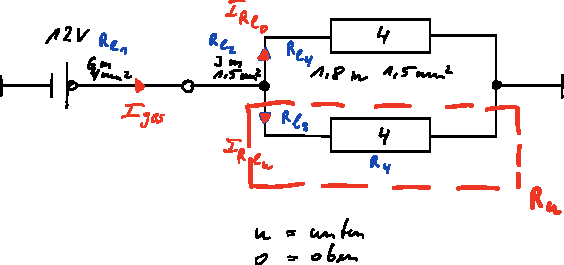
\includegraphics[width=0.6\textwidth]{images/Skizze/25_FM_Nr7_gemischte_Schaltung_A2.pdf}
\caption{FM Nr7 gemischte Schaltung A2}
%\label{fig:}%% anpassen
\end{figure}

\lstset{language=Python}% C, TeX, Bash, Python 
\begin{lstlisting}[
	%caption={}, label={code:}%% anpassen
][language=Python]
# geg: Schaltung
U_ges = 12 V
l_1 = 6 m
A_1 = 4 mm^2
l_2 = 3 m
A_2 = 1,5 mm^2
l_3 = 1,8 m
A_3 = 1,5 mm^2
R_4 = 4 Ohm
p = 0,0178 Kupfer ohm x mm^2 / m 
# ges: U_v_Leitung
# Formel:
R_l_1 = p x l_1 / A_1
R_l_2 = p x l_2 / A_2
R_l_3 = p x l_3 / A_3
R_u = R_l_3 + R_4 (R_o = R_u)
R_II = R_u/2
R_ges = R_l_1 + R_l_2 + R_II
I_ges = U_ges/R_ges
U_v_R_l_3 = R_l_3 x I_R_l_3 -> U_v_R_l_3 = (R_l_3 x I_ges)/2
# Lösung:
R_l_1 = 0,0267 Ohm
R_l_2 = 0,0356 Ohm
R_l_3 = 0,0214 Ohm
R_u = 4,0214 Ohm
R_l_1 = 0,0267 Ohm
R_II = 2,0107 Ohm
R_ges = 2,073 Ohm
I_ges = 5,7888 A
U_v_R_l_3 = 0,0618 V
\end{lstlisting}

\newpage

\textbf{Aufgabe 3}

\begin{figure}[!ht]% hier: !ht
\centering
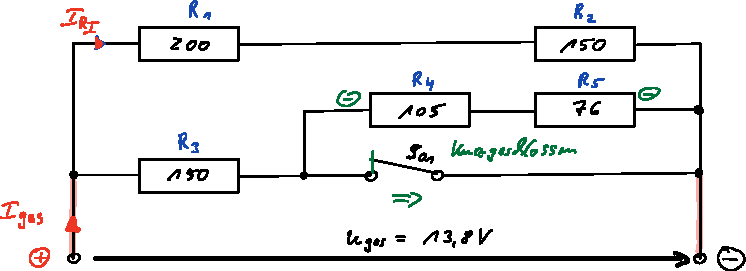
\includegraphics[width=0.6\textwidth]{images/Skizze/25_FM_Nr7_gemischte_Schaltung_A3.pdf}
\caption{FM Nr7 gemischte Schaltung A3}
%\label{fig:}%% anpassen
\end{figure}

\lstset{language=Python}% C, TeX, Bash, Python 
\begin{lstlisting}[
	%caption={}, label={code:}%% anpassen
][language=Python]
# geg: Schaltung
R_1 = 200 Ohm
R_2 = 150 Ohm
R_3 = 150 Ohm
R_4 = 105 Ohm
R_5 = 76 Ohm
U_ges = 13,8 V
# Formel:
# 3,1) ges: R_I, R_II, R_ges_1, R_ges_2, R_delta
R_I = R_1 + R_2
R_II = R_3 + R_4 + R_5 (Schalter offen)
R_ges_1 = 1/(1/R_I + 1/R_II) (Schalter offen)
R_ges_2 = 1/(1/R_II + 1/R_3) (Schalter zu)
R_delta = R_ges_1 - R_ges_2
Gesamtwiderstand ändert sich
# 3,3) ges: I_R_3
I_R_3 = U_ges/R_II (Schalter offen)
# 3,4) ges: U_S_01
U_S_01 = (R_4 + R_5) x I_R_3 (Schalter offen)
# 3,5) ges: I_R_1
I_R_1 = U_ges/R_I
Strom bleibt immer gleich, egal ob Schalter auf/zu
# Lösung:
R_I = 350 Ohm
R_II = 331 Ohm
R_ges_1 = 170,1175 Ohm
R_ges_2 = 103,2225 Ohm
R_delta = 66,895 Ohm
I_R_3 = 0,0417 A
U_S_01 = 7,5462 V
I_R_1 = 0,0394 A
\end{lstlisting}

\newpage

\textbf{Aufgabe 4}

\begin{figure}[!ht]% hier: !ht
\centering
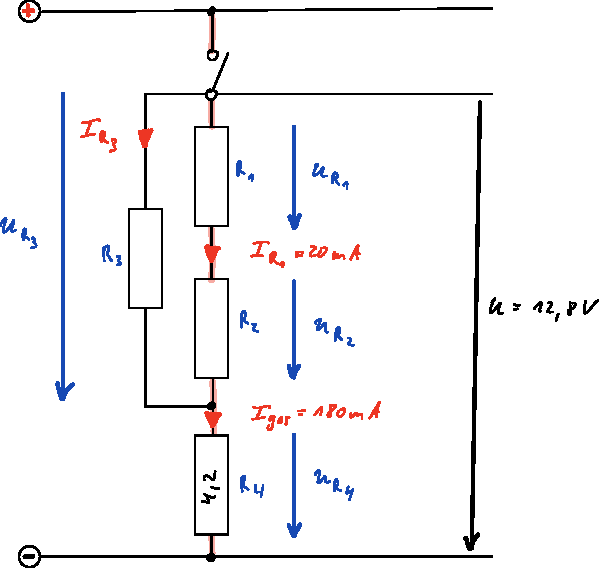
\includegraphics[width=0.6\textwidth]{images/Skizze/25_FM_Nr7_gemischte_Schaltung_A4.pdf}
\caption{FM Nr7 gemischte Schaltung A4}
%\label{fig:}%% anpassen
\end{figure}

\lstset{language=Python}% C, TeX, Bash, Python 
\begin{lstlisting}[
	%caption={}, label={code:}%% anpassen
][language=Python]
# geg: Schaltung
R_4 = 4,2 Ohm
U_ges = 12,8 V
U_R_2 = 1,65 V
I_R_1 = 0,02 A = 20 mA
I_ges = 0,18 A = 180 mA
# ges: R_2, U_R_4, R_1, R_3
# Formel:
R_2 = U_R_2/I_R_1
U_R_4 = R_4 x I_ges
R_1 = U_R_1/I_R_1 -> R_1 = (U_ges - U_R_2 - U_R_4)/I_R_1
R_3 = U_R_3/I_R_3 -> R_3 = (U_ges - U_R_4)/(I_ges - I_R_1)
# Lösung:
R_2 = 82,5 Ohm
U_R_4 = 0,756 V
R_1 = 519,7 Ohm
R_3 = 75,275 Ohm
\end{lstlisting}
 \newpage
%ju 28-Mai-22 FM_U08_Leistung_Loesung.tex
\section{Leistung Übung 8}\label{leistung-uebung-8}

\textbf{Aufgabe 1}

\begin{figure}[!ht]% hier: !ht
\centering
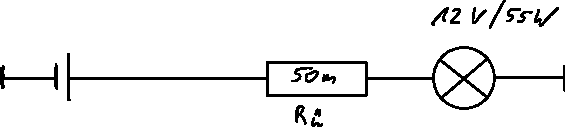
\includegraphics[width=0.6\textwidth]{images/Skizze/26_FM_Nr8_Leistung_A1.pdf}
\caption{FM Nr8 Leistung A1}
%\label{fig:}%% anpassen
\end{figure}

\lstset{language=Python}% C, TeX, Bash, Python 
\begin{lstlisting}[
	%caption={}, label={code:}%% anpassen
][language=Python]
# geg:
U_ges = 14,8 V
R_u = 0,05 Ohm = 50 mOhm
P_La = 55 W
U = 12 V
# ges: P_La_tat
# Formel:
P_La = U x I -> P_La = U^2/R_La -> R_La = U^2/P_La
R_ges = R_u + R_La
I_tat = U_ges/R_ges
P_La_tat = U_k x I_tat -> P_La_tat = R_La x I_tat^2
# Lösung:
R_La = 2,6182 Ohm
R_ges = 2,6682 Ohm
I_tat = 5,5468 A
P_La_tat = 80,555 W
\end{lstlisting}

\textbf{Aufgabe 2}

\lstset{language=Python}% C, TeX, Bash, Python 
\begin{lstlisting}[
	%caption={}, label={code:}%% anpassen
][language=Python]
# geg:
R = 50 Ohm
P = 500 W
# ges: I
# Formel:
P = U x I -> P = R x I^2 -> I = sqrt(P/R)
# Lösung:
I = 3,1623 A
\end{lstlisting}

\newpage

\textbf{Aufgabe 3}

\begin{figure}[!ht]% hier: !ht
\centering
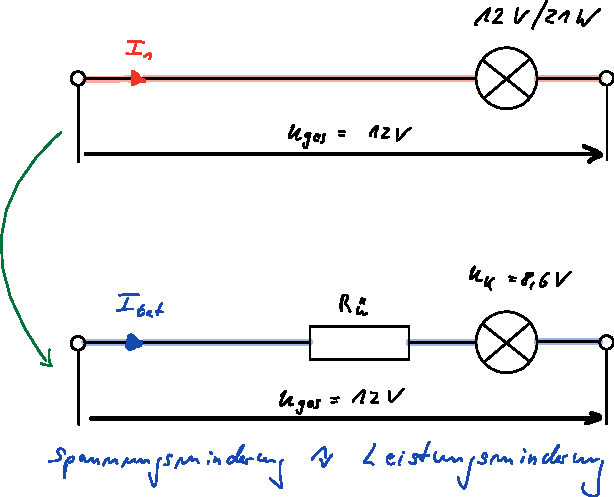
\includegraphics[width=0.6\textwidth]{images/Skizze/26_FM_Nr8_Leistung_A3.pdf}
\caption{FM Nr8 Leistung A3}
%\label{fig:}%% anpassen
\end{figure}

\lstset{language=Python}% C, TeX, Bash, Python 
\begin{lstlisting}[
	%caption={}, label={code:}%% anpassen
][language=Python]
# geg:
U_ges = 12 V
P_La = 21 W
U_k = 8,6 V
# ges: R_u, P_R_u, P_La_tat
# Formel:
P_La = U x I -> P_La = U^2/R_La -> R_La = U_ges^2/P_La
I_tat = U_k/R_La
R_u = U_R_u/I_tat -> R_u = (U_ges - U_k)/I_tat
P_R_u = U_R_u x I_tat ->
P_R_u = R_u x I_tat^2
P_La_tat = U_k x I_tat
# Lösung:
R_La = 6,8571 Ohm
I_tat = 1,2542 A
R_u = 2,711 Ohm
P_R_u = 4,2642 W
P_La_tat = 10,7858 W
\end{lstlisting}

\newpage

\textbf{Aufgabe 4}

\textbf{Durch welche technische Größe kommt es bei einer 24 V Glühlampe
zur gleichen Leistung wie bei einer 12 V Glühlampe, obwohl doch die
äußerlichen Baugrößen identisch sind?}

\begin{figure}[!ht]% hier: !ht
\centering
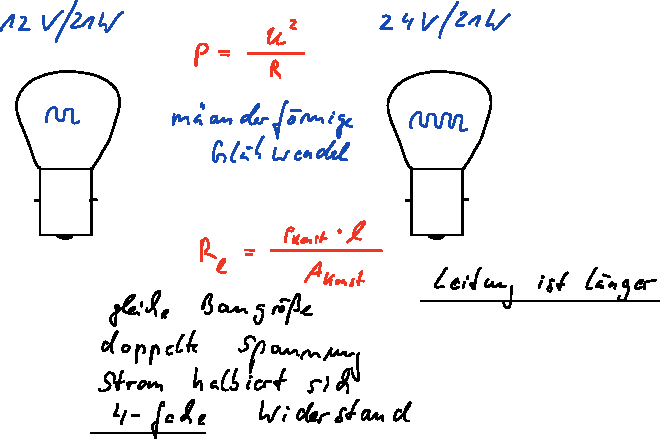
\includegraphics[width=0.6\textwidth]{images/Skizze/26_FM_Nr8_Leistung_A4.pdf}
\caption{FM Nr8 Leistung A4}
%\label{fig:}%% anpassen
\end{figure}

\lstset{language=Python}% C, TeX, Bash, Python 
\begin{lstlisting}[
	%caption={}, label={code:}%% anpassen
][language=Python]
# geg:
P = 21 W
U_1 = 12 V
U_2 = 24 V
# Formel:
P = U x I -> P = U^2/R ->
R_1 = U_1^2/P
R_2 = U_2^2/P
Faktor = R_2/R_1
# Lösung:
12V/21W R_1 = 6,8571 Ohm
24V/21W R_2 = 27,4286 Ohm
Faktor = 4 - fache Widerstand
\end{lstlisting}

Bei einer 24 V Lampe ist der Widerstand viermal größer als bei einer 12
V Glühlampe. Dieser Widerstand liegt hierbei an einer doppelten Spannung
gegenüber der 12 V Spannung. Durch die doppelte Spannung und dem
vierfachen Widerstand stellt sich ein Strom ein, der die Hälfte
gegenüber einer Spannung von 12 V hat.

Somit ergibt sich die gleiche Leistung bei 24 V. Um diesen Widerstand zu
erhalten, vierfache Leiterlänge, ist die Glühwendel mäanderförmig
gefertigt in dem Glaskolben verlegt.

\textbf{Aufgabe 5}

\textbf{Wenn man ein 12 V Bordnetz mit einem 24 V Bordnetz vergleicht,
stellt man in der Dimensionierung der verlegten elektrischen Leitung
kein Unterschied fest. Ist die oben genannte Aussage zutreffend, oder
gibt es ihrer Meinung nach doch ein Unterschied in der Dimensionierung
der Leitungen?}

Die Spannung ist höher, demzufolge kann die Stromstärke kleiner sein,
ergo können auch die Leitungen in ihrer Fläche kleiner sein, da die
Belastung nicht so groß ist.

Da der Stromfluss durch die Leitungen geringer ist, tritt an diesen
Leitungen auch nicht ein so großer Spannungsverlust auf. Dadurch tritt
an dem zu schaltenden Verbraucher auch nicht eine so hohe
Spannungsminderung der Klemmenspannung auf.
 \newpage
%ju 28-Mai-22 FM_U08_Leistung_Mathebuch_Loesung.tex
\section{Leistung Übung 8
Mathebuch}\label{leistung-uebung-8-mathebuch}

Vgl. Mathebuch (\textcite{elbl:2016:technMa})

\textbf{S. 82 Aufgabe 4d}

\lstset{language=Python}% C, TeX, Bash, Python 
\begin{lstlisting}[
	%caption={}, label={code:}%% anpassen
][language=Python]
# geg:
I_ges = 0,35 A
U = 210 V
R_2 = 1000 Ohm = 1 k
# ges: I_1, I_2, R_ges, R_1, P_R_1, P_R_2
# Formel:
R_ges = U/I_ges
I_2 = U/R_2
I_ges = I_1 + I_2 -> I_1 = I_ges - I_2
R_1 = U/I_1
P_R_1 = U x I_1
P_R_2 = U x I_2
# Lösung:
R_ges = 600,0 Ohm
I_2 = 0,21 A
I_1 = 0,14 A
R_1 = 1500,0 Ohm
P_R_1 = 29,4 W
P_R_2 = 44,1 W
\end{lstlisting}

\textbf{S. 84 Aufgabe 4}

\lstset{language=Python}% C, TeX, Bash, Python 
\begin{lstlisting}[
	%caption={}, label={code:}%% anpassen
][language=Python]
# geg: Glühkerze
U_k = 10,5 V
P_k = 100 W
# ges: I_k, R_k
# Formel:
P = U x I -> I_k = P_k/U_k
R_k_1 = U_k/I_k (Var, 1)
P = U x I -> P = U^2/R
R_k_2 = (U_k x U_k)/P_k (Var, 2)
# Lösung:
I_k = 9,5238 A
R_k_1 = 1,1025 Ohm
R_k_2 = 1,1025 Ohm
\end{lstlisting}

\newpage

\textbf{S. 82 Aufgabe 3}

\begin{figure}[!ht]% hier: !ht
\centering
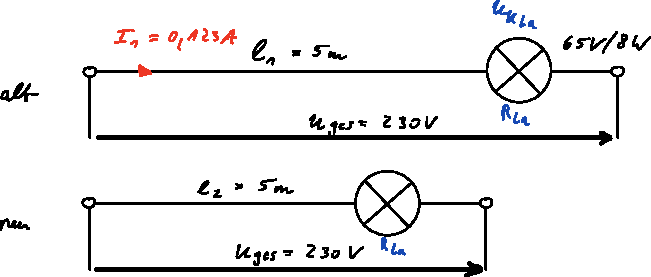
\includegraphics[width=0.6\textwidth]{images/Skizze/26_FM_Leistung_Mathebuch_A3.pdf}
\caption{FM Leistung Mathebuch A3}
%\label{fig:}%% anpassen
\end{figure}

\lstset{language=Python}% C, TeX, Bash, Python 
\begin{lstlisting}[
	%caption={}, label={code:}%% anpassen
][language=Python]
# geg: Leuchtstoffröhre 65V/8W Schaltung
U_ges = 230 V
U_k_La = 65 V
l_1 = 5 m
l_2 = 4 m
I_1 = 0,123 A = 123 mA
# ges: U_k_La_tat, P_La_tat
# Formel:
R_La = U_k_La/I_1
# R_l_1 = U_R_l_1/I_1
R_l_1 = (U_ges - U_k_La)/I_1
# Dreisatz
5 m = 1341,46 Ohm
4 m = x Ohm
R_l_2 = l_2 x R_l_1/l_1
R_ges_tat = R_l_2 + R_La
I_tat = U_ges/R_ges_tat
U_k_La_tat = R_La x I_tat
P_La_tat = U_k_La_tat x I_tat
# Lösung:
R_La = 528,4553 Ohm
R_l_1 = 1341,4634 Ohm
R_l_2 = 1073,1707 Ohm
R_ges_tat = 1601,626 Ohm
I_tat = 0,1436 A
U_k_La_tat = 75,8883 V
P_La_tat = 10,8979 W
\end{lstlisting}
 \newpage


\chapter{FT - Übungen}
%ju 28-Mai-22 FT_U09_VW_Stromlaufplan_Motronic2l_AZJ_Loesung.tex
\section{Aufgabenstellung Messübungen Motronic 2,0l
AZJ}\label{aufgabenstellung-messuebungen-motronic-20l-azj}

\textbf{(Ü9) Aufgabenstellung und VW Stromlaufplan S. 1-3 Erklärung}

$\to$ vom Ziel zurück zur Batterie/Generator lesen

$\to$ Elektrische Ladungen gleichen sich grundsätzlich immer dort aus,
wo sie getrennt worden sind!

$\to$ Ein elektrischer Strom kann grundsätzlich immer nur in einem
geschlossenen Stromkreis fließen.

\textbf{Aufgabe 1}

Ja, die Aussage ist zutreffend. Strompfad 101-107

\begin{itemize}
\item
  S223 Sicherung im Strompfad 99, rot, 10 A
\item
  und S163 Sicherung Strompfad 8, rot 50 A
\end{itemize}

\emph{Farben der Sicherungen} Vgl. Tabellenbuch
(\textcite{bell:2021:tabellenbuchKfz} S. 281)

\textbf{Aufgabe 2}

S243 Sicherung Strompfad 156, über die Trennstelle T4f/1 Strompfad 112
erfolgt die positive Spannungsversorgung.

\textbf{Aufgabe 3}

Kl. 3/86 + auf Kl. 5/85 - messen, Bordnetzspannung beträgt 13,8 V

Die Spannung, die am Steuerstrom Anschluss gemessen werden kann, beträgt
4,6 V.

\emph{Alternative:} die Gesamtspannung durch die Anzahl der Widerstände
dividieren. Hier in diesem Fall haben wir es mit drei gleich große
Widerstände zu tun.

3x gleich große Widerstände a $72~\Omega \quad$
$U_{Teil} = \frac{13,8~V}{3} = 4,6~V$

\textbf{Aufgabe 4}

Ja, sie werden durch zwei verschiedene Sicherungen abgesichert.

\begin{itemize}
\item
  Komponente N156 S10 mit 15 A, Strompfad 19
\item
  Komponente N261 S234 mit 10 A Strompfad 157
\end{itemize}

\textbf{Aufgabe 5}

Es wird gegen PIN1 und PIN4 jeweils ein positiver Spannungswert von 13,8
V gemessen (Bordnetzspannung), es fließt in der jetzigen Situation kein
Strom, demzufolge kann auch an der Sicherung keine Spannung abfallen.

Das \emph{Spannungsmessgerät} wird mit dem \emph{roten Clip} an PIN1
kabelbaumseitig von G6, der \emph{schwarze Clip} an PIN4 und PIN1 von G6
angeschlossen, es wird dann ein positiver Spannungswert angezeigt.

\textbf{Aufgabe 6}

Die Zündspule mit Leistungsendstufen im Strompfad 30 - 42 werden über
die Trennstelle T6d/1 mit negativem Potenzial versorgt. Die Verbindung
mit Masse erfolgt im Strompfad 180.

Masseverbindung ist im Strompfad 180 auf Masse geschadet/gelegt.

\textbf{Aufgabe 7}

\lstset{language=Python}% C, TeX, Bash, Python 
\begin{lstlisting}[
	%caption={}, label={code:}%% anpassen
][language=Python]
# geg:
U_B = 13,8 V
U_CE = 1,5 V
R_Ventil = 17 Ohm
# ges: P_E-Ventil_1.Zyl
# Formel:
I = U_Ventil / R_Ventil -> I = (U_B - U_CE) / R_Ventil
P = U x I -> P = (U_B - U_CE) x I
# Lösung:
I = 0,7235 A
P = 8,8994 W
\end{lstlisting}

\textbf{Aufgabe 8}

\lstset{language=Python}% C, TeX, Bash, Python 
\begin{lstlisting}[
	%caption={}, label={code:}%% anpassen
][language=Python]
# geg:
U_B = 13,8 V
U_CE = 1,5 V
R_Ventil = 17 Ohm
A = 0,35 mm^2 aus Stromlaufplan Nr. 77/9
l = 1,2 m
p = 0,0178 Ohm x mm^2/m
# ges: Spannungsminderung U_v_minusseitigeVersorgung_4.Zyl
# Formel:
U_Ventil = U_B - U_CE - U_v
R_l = p x l / A
R_ges = R_Ventil + R_l
I = U_k / R_ges -> I = (U_B - U_CE) / R_ges
U_v = I x R_l
# Alternative
U_v = I x p x l / A
# Lösung:
R_l = 0,061 Ohm
R_ges = 17,061 Ohm
I = 0,7209 A
U_v = 0,044 V
\end{lstlisting}

\textbf{Aufgabe 9}

\begin{enumerate}
\item
  Steuerstrom Kraftstoffpumpenrelais J17 (grün)

  \begin{itemize}
  \item
    Stromlaufplan S. 2,3,11,12,13,2
  \end{itemize}
\item
  Steuerstrom Relais J299 für Sekundärluftpumpe (rot)

  \begin{itemize}
  \item
    Stromlaufplan S. 2, \ldots{} , 11,12,13,5
  \end{itemize}
\item
  Laststrom Relais J299 für Sekundärluftpumpe, Laststrom V101 (blau)

  \begin{itemize}
  \item
    Stromlaufplan S. 2,12
  \end{itemize}
\end{enumerate}

\textbf{Aufgabe 10}

V101 - Motor für Sekundärluftpumpe

Das Bauteil ist durch die Sicherung S162 im Sicherungshalter/Batterie
(50 A) abgesichert. Strompfad 6 Stromlaufplan S. 12.
 \newpage
%ju 28-Mai-22 FT_U10_VW_Stromlaufplan_Beleuchtungssystem_Loesung.tex
\section{Übungsaufgaben
Beleuchtungssystem}\label{uebungsaufgaben-beleuchtungssystem}

\textbf{(Ü10) Scheinwerferhöhenverstellung Beleuchtungssystem + VW
Stromlaufplan}

\textbf{Aufgabe 1}

\begin{itemize}
\item
  Ist eine Wartung durchgeführt worden?
\item
  Ist die Glühlampe oder der Scheinwerfer gewechselt worden
\item
  ist eine Motorwäsche durchgeführt worden
\item
  unter welchen Bedingungen ist dieses Ereignis aufgetreten
  (Feuchtigkeit, Wetter)
\item
  Unfall (Quetschung der Leitungen, Übergangswiderstand bilden)
\item
  witterungsbedingte Einflussnahme
\end{itemize}

\textbf{Aufgabe 2} Messung Strompfad 186-196 (Schaltplan VW -
Scheinwerferhöhenverstellung Beleuchtungssystem)

\begin{figure}[!ht]% hier: !ht
\centering
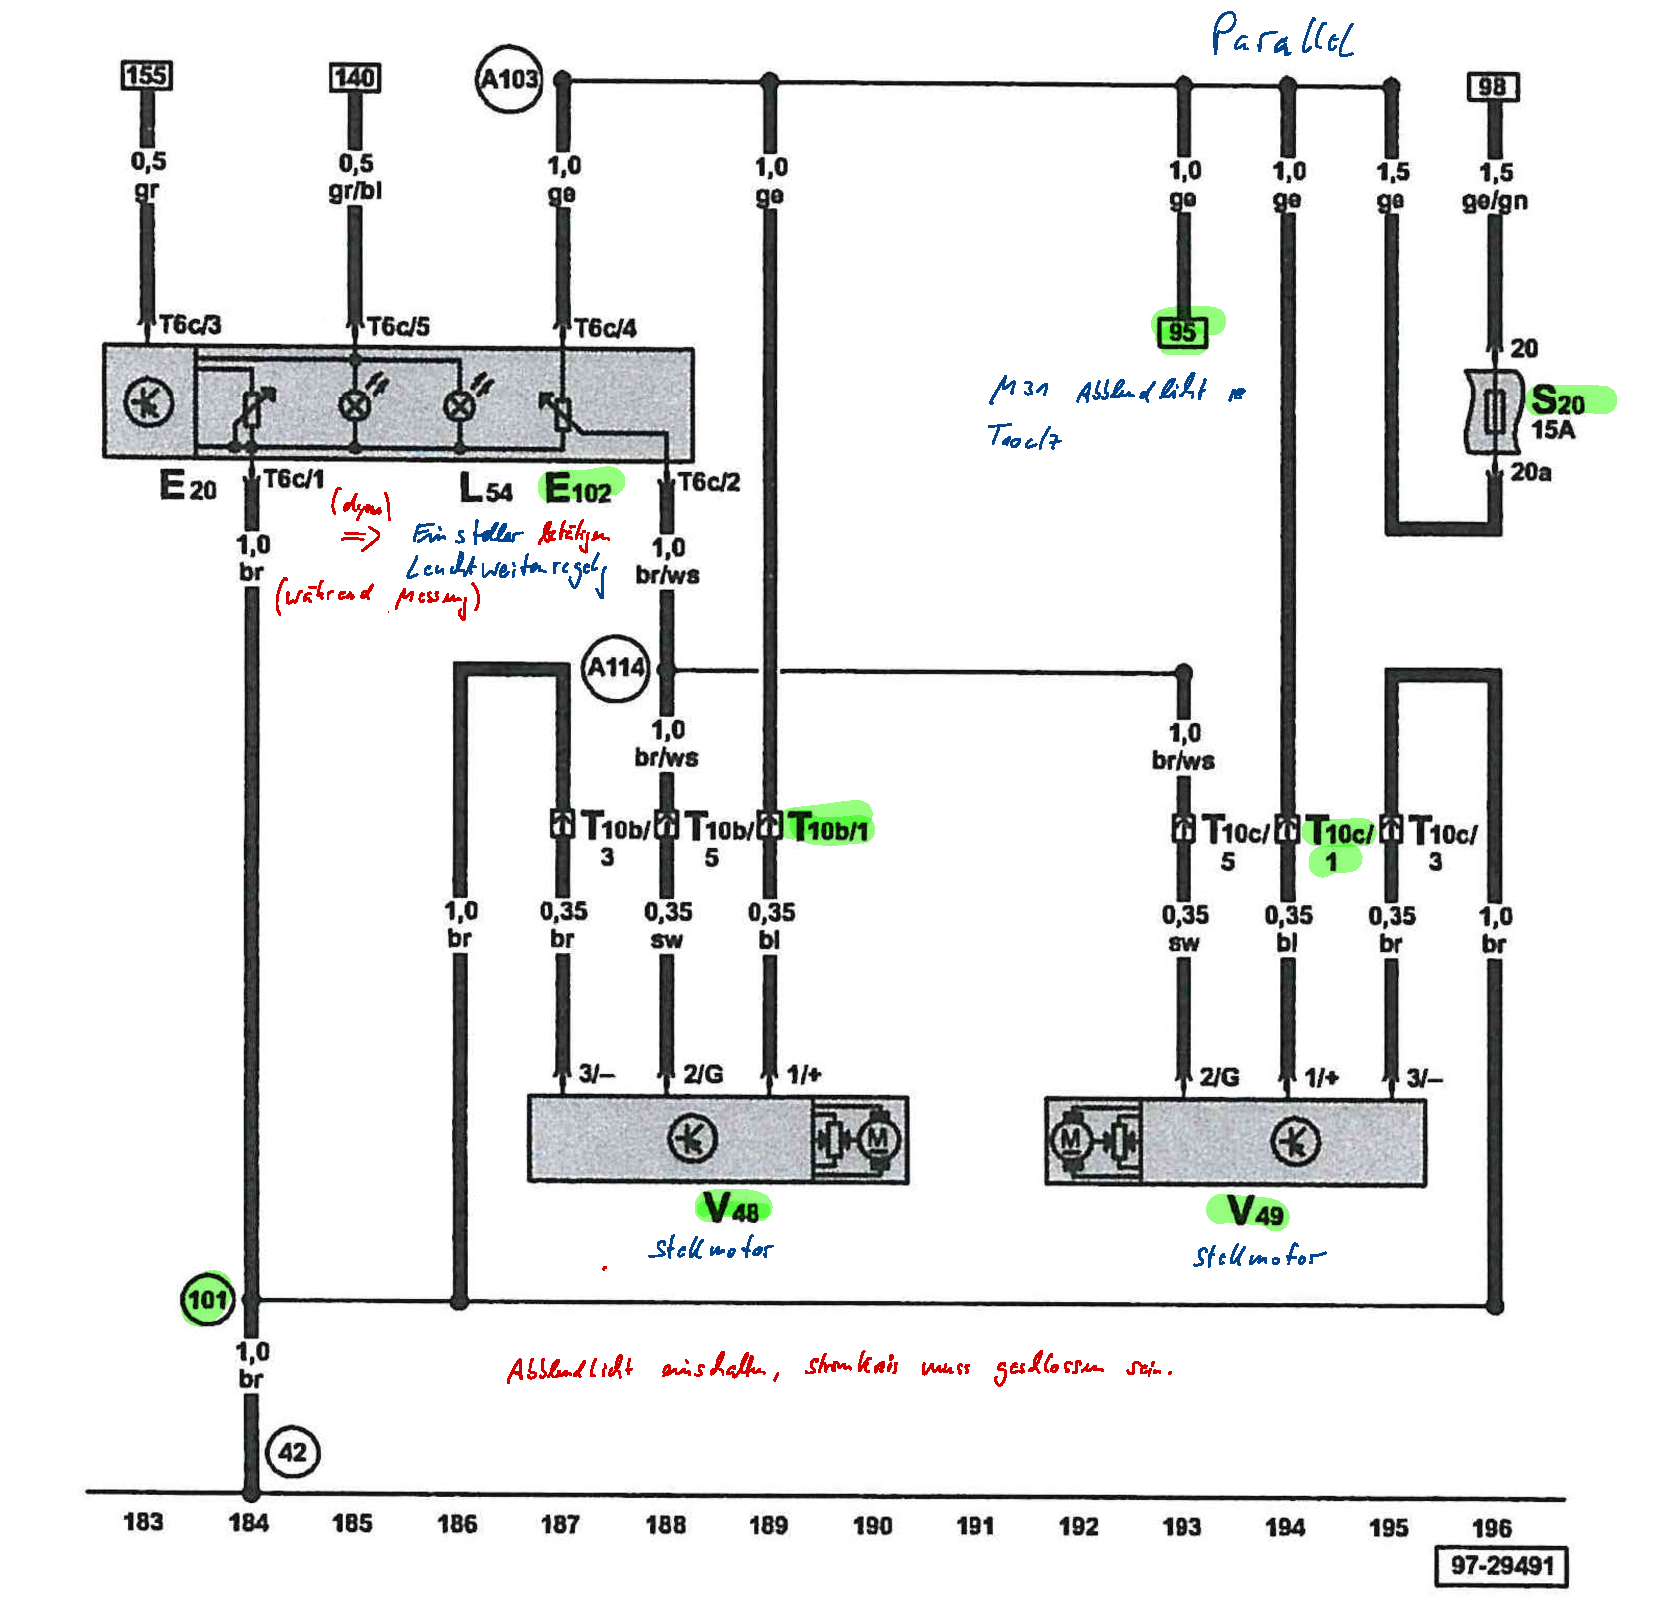
\includegraphics[width=0.9\textwidth]{images/Skizze/28_Scheinwerferhoehenverstellung.pdf}
\caption{Scheinwerferhöhenverstellung}
%\label{fig:}%% anpassen
\end{figure}

\begin{itemize}
\item
  Klemmenspannung Stellmotor messen
\item
  Geberspannung Signal (hoch/runter) messen
\item
  Synchronisierung der Höhenverstellung durchführen
\item
  mit Diagnosetester Fehlerspeicher auslesen
\item
  Sichtprüfung Stecker, Leitung, Sicherung, Mechanik
\end{itemize}

\textbf{Aufgabe 3} Ausgangszustand ist eine abgeglichene
Brückenschaltungsspannung zwischen dem Potenziometer E102 und
Potenziometern der Scheinwerfermotoren V48 und V49. Wird die
Potentiometerstellung (Stellrad) an E102 geändert, ändert sich
automatisch die Brückenspannung zwischen den beiden Komponenten \{E102
und den Potis von V48 und V49\}.

Die Auswerteelektronik erfasst im Brückenspannungswert und steuert die
Motoren V48 und V49 so lange mit der entsprechenden Polarität an, bis
die Brückenspannung wieder den Wert Null Volt erreicht. Die
Brückenspannung hat jetzt wieder ihren Ausgangswert (0 V), allerdings
bei einer anderen Stellung der Reflektoren.

Als Information über den Drehwinkelstand der Motoren, dienen die
Potenziometer, deren Schleifer mit den Reflektoren verbunden sind.

Das Bauteil, welches in der Regel verstellt wird, ist der Reflektor.

Die Drehrichtungsänderung erfolgt über die Polaritätsänderung an den
elektrischen Anschlüssen der Motoren.

\textbf{Aufgabe 4} Messobjekt (Poti E102) muss aus dem Stromkreis gelöst
und spannungsfrei sein.

Zur Messung des Wiederstandes Poti gemäß seiner Funktion
bewegen/drehen/verändern alle Funktionen/Stufen durchschalten.

\textbf{Aufgabe 5} Fahrzeuge mit Xeon Scheinwerfersystemen müssen mit
einer

\begin{enumerate}
\item
  automatischen Scheinwerferhöhenverstellungeinrichtung und
\item
  mit einer Scheinwerferreinigungsanlage ausgestattet sein,
\item
  bei Scheinwerfern mit Gasentladungslampen für Abblendlicht, wenn
  hierbei das Fernlicht eingeschaltet wird, muss das Abblendlicht in
  Funktion bleiben, also eingeschaltet bleiben
\end{enumerate}

siehe §50 STVZO, Tabellenbuch D2S, D2R, D1S, D1R

Scheinwerferhöhenverstellung

\begin{itemize}
\item
  Manuell
\item
  Automatisch
\item
  Dynamisch
\item
  Stichwort: Scheinwerferreinigungsanlage
\end{itemize}

\textbf{Aufgabe 6}

\begin{itemize}
\item
  Die Geräte M29, M31, V48 und V49 sind schaltungstechnisch parallel
  geschaltet, wobei M29 über die Sicherung S21 abgesichert wird,
  insofern hier keine Spannungsminderung auftreten wird
\item
  die Geräte M31 T10c/7, V48 T10b/1, V49 T10c/1, als auch E102 erfahren
  die Spannungsminderung um 3,25 V (alles auf die Masseversorgung des
  jeweiligen Bauteils gemessen)
\item
  Der Stromkreis muss geschlossen sein, es muss ein Strom fließen, also
  Licht (Abblendlicht) einschalten!
\item
  Einsteller E102 während der Messung betätigen
\end{itemize}

\textbf{Aufgabe 7}

Prüfzeichen und Bauartgenehmigung für Fahrzeugteile §21a, §22a

\begin{itemize}
\item
  \textbf{BRD} \verb|\~\~\~|
\item
  \textbf{EG} e1
\item
  \textbf{ECE} E1 (Prüfbuchstabe, Genehmigungsnummer, 1 = Deutschland, 2
  = Frankreich)
\end{itemize}

\textbf{Aufgabe 8}

Stromlaufplan Nr. 73/2 + 73/12 + 73/8 + 73/15

\begin{enumerate}
\item
  (Farbe Rot) Leuchtweitenregulierungsverlauf
\item
  (Farbe Blau) Laststrom Motoren Leuchtweiten
\item
  (Farbe Grün) Stromverlauf Abblendlicht
\end{enumerate}

\newpage

\textbf{Aufgabe 9}

Schaltbild

\begin{figure}[!ht]% hier: !ht
\centering
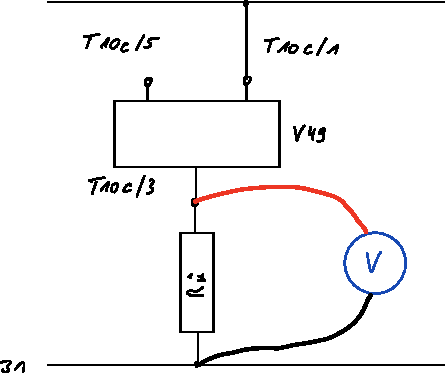
\includegraphics[width=0.6\textwidth]{images/Skizze/29_FT_minusseitiger_Ubergangswiderstand.pdf}
\caption{minusseitiger Übergangswiderstand}
%\label{fig:}%% anpassen
\end{figure}

Es hat sich zwischen T10c/3 und der Masseverbindung im Leitungsstrang
Strompfad 184 ein Übergangswiderstand gebildet, er liegt in Reihe zum
V49. Dieser Widerstand mindert die Klemmenspannung des Motors V49,
ferner bekommt die Brückenschalung des V49 unplausible Widerstandswerte.
Man spricht hierbei von einem minusseitigen Übergangswiderstand. Der
Spannungsverlust, der hierbei entsteht, bezeichnet man als einen
minusseitigen Spannungsverlust.

\begin{table}[!ht]% hier: !ht 
\centering 
	\caption{}% \label{tab:}%% anpassen 
\begin{tabular}{@{}ll@{}}
\hline
\textbf{Bezeichnung} & \textbf{Benennung} \\
\hline
V49 & Scheinwerferhöhenverstellmotor rechts \\
T10c/5 & Anschluss Steuerung \\
T10c/1 & Plusversorgung \\
T10c/3 & Masse \\
$R_\text{ü}$ & Übergangswiderstand \\
\hline
\end{tabular} 
\end{table}

\newpage

\textbf{Aufgabe 10}

\lstset{language=Python}% C, TeX, Bash, Python 
\begin{lstlisting}[
	%caption={}, label={code:}%% anpassen
][language=Python]
# geg:
P_M_31 = 55 W/12V
U = 12 # V
U_ges = 14,3 V
U_v = 3,25 V
# ges: P_M_31_tat
# Formel:
P_M_31 = U x I -> I = P_M_31 / U
R = U / I
I_tat = U_k / R -> I_tat = (U_ges - U_v) / R
P_M_31_tat = U_k x I_tat -> P_M_31_tat = (U_ges - U_v) x I_tat
# Lösung:
I = 4,5833 A
R = 2,6182 Ohm
I_tat = 4,2205 A
P_M_31_tat = 46,6364 W
\end{lstlisting}

\textbf{Aufgabe 11}

d = 31, 56a, 56b, 58R (Scheinwerfer vorne rechts)

\newpage

\textbf{Aufgabe 12}

\lstset{language=Python}% C, TeX, Bash, Python 
\begin{lstlisting}[
	%caption={}, label={code:}%% anpassen
][language=Python]
# geg:
P_12 = 21 W/12V
P_24 = 21 W/24V
U_12 = 12 V
U_24 = 24 V
# ges: R_24, R_12
# Formel:
P_12 = U x I -> I_12 = P_12 / U_12
R_12 = U_12 / I_12
P_24 = U x I -> I_24 = P_24 / U_24
R_24 = U_24 / I_24
Faktor = R_24 / R_12
# Lösung:
I_12 = 1,75 A
R_12 = 6,8571 Ohm
I_24 = 0,875 A
R_24 = 27,4286 Ohm
Faktor 12V / 24V = 4,0 -fache Leiterlaenge
\end{lstlisting}

Bei einer 24 V Glühlampe ist der Widerstand viermal größer (vierfache
Leiterlänge) als bei einer 12 V Glühlampe. Dieser Widerstand liegt
hierbei an einer doppelten Spannung gegenüber der 12 V Spannung. Durch
die doppelte Spannung und dem vierfachen Widerstand ergibt sich eine
gleiche Leistung, bei gleicher Baugröße des Glaskolbens. Um diesen
Widerstand in die gleiche Glaskolbengröße hineinzubekommen, ist die
Glühwendel mäanderförmig gefertigt, im Glaskolben verlegt.

\textbf{Aufgabe 13}

siehe Musterlösung
 \newpage



%\chapter{x-PDFs}
% ju 28-Nov-2021 PDFs.tex 

\chapter{Messen}\label{sec:Messen}\index{Messen}


% -------
\section{Messmethodik - Schaltkreis}\label{sec:Messmethodik_Schaltkreis}\index{Messmethodik_Schaltkreis}
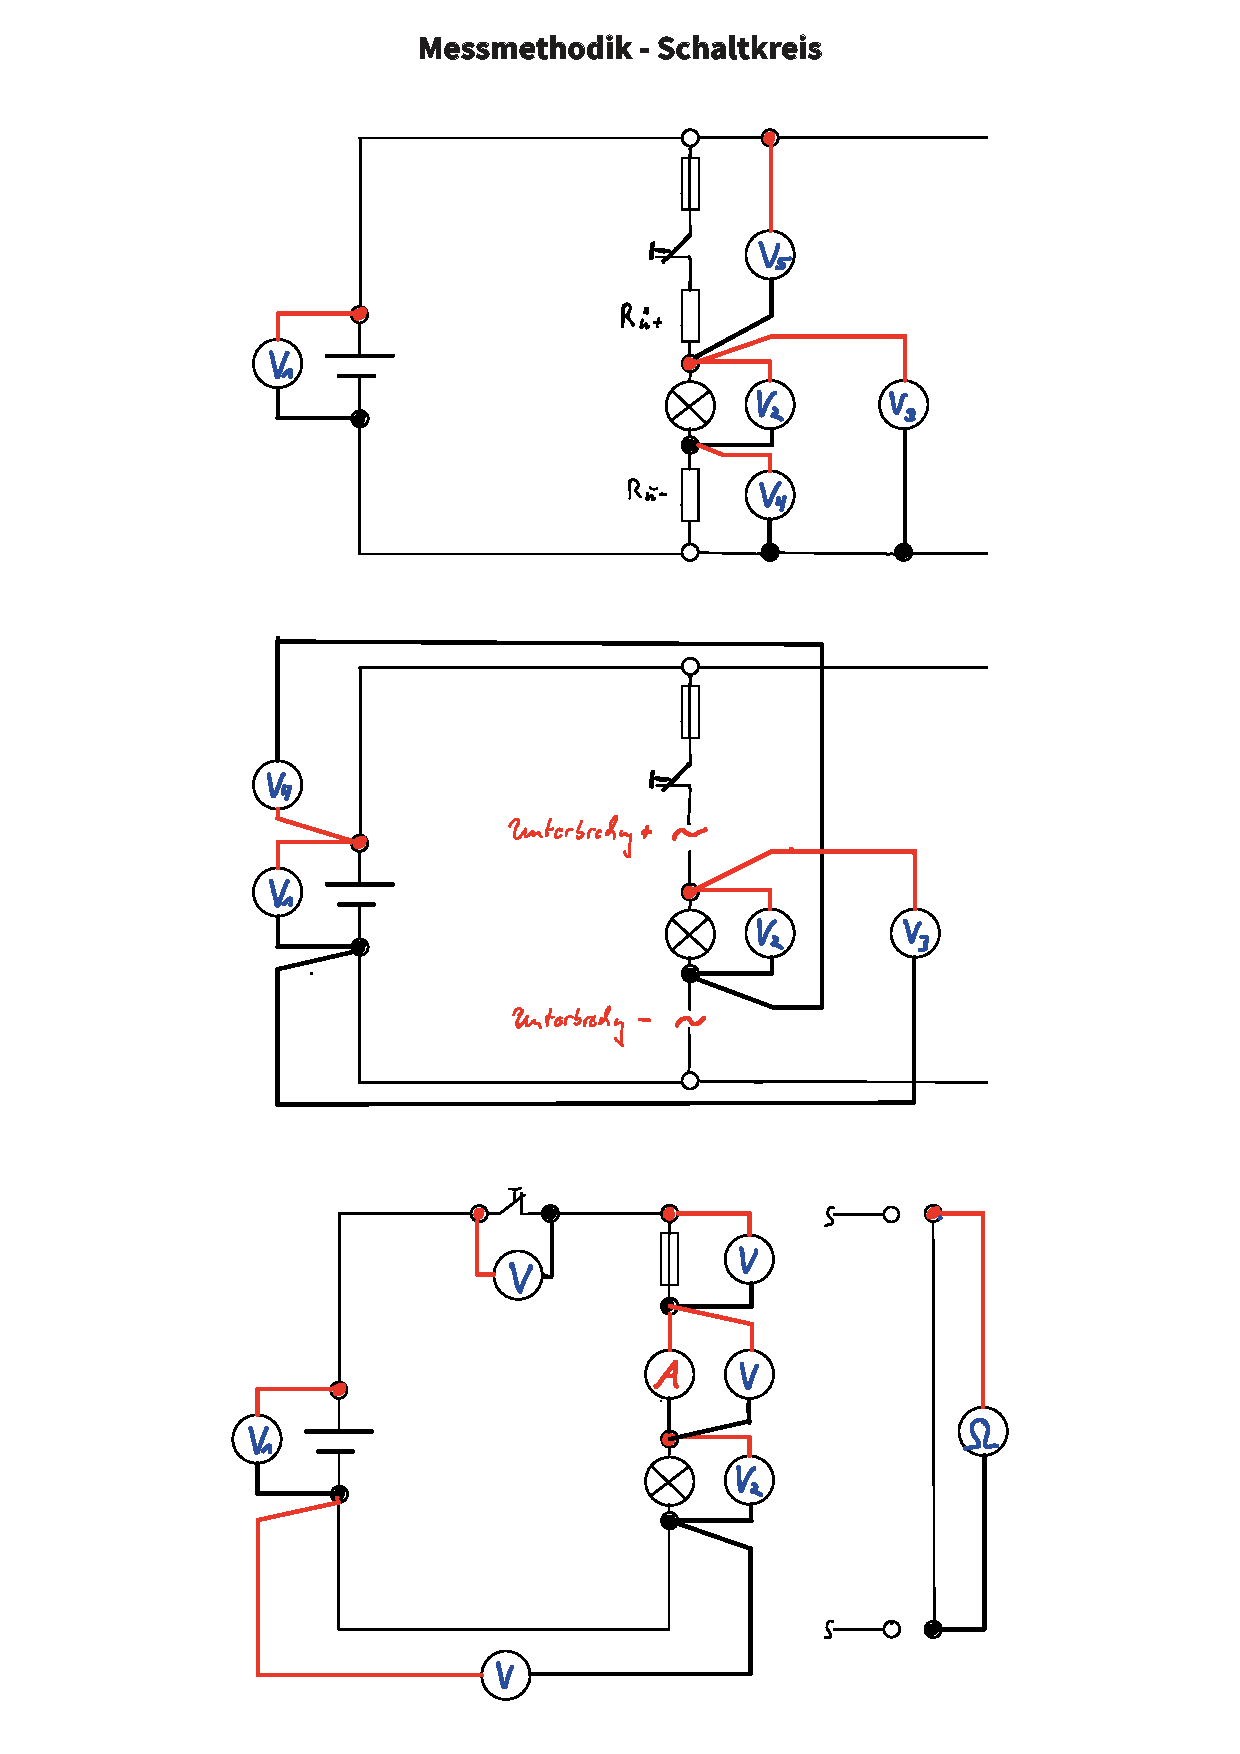
\includepdf[pages=-]{Tabellen/PDF/Messmethodik-Schaltkreis.pdf}

% -------
\section{Messprotokoll}\label{sec:Messprotokoll}\index{Messprotokoll}
\includepdf[pages=-]{Tabellen/PDF/Messprotokoll.pdf}






%%%%%%%%%%%%%%%%%%%%%%%%%%%%%%%%%%%%%%%%%%%%%%%%%%